\chapter{Isoform landscape of AD-associated genes from targeted profiling of tau mouse model}\label{ch: targeted_transcriptome}
\label{targetedmousetranscriptome}

%https://www.frontiersin.org/articles/10.3389/fmolb.2021.711733/full

\section{Introduction}
Long-read sequencing of the whole transcriptome at a global level provide valuable insights into the role of splicing and RNA isoforms in health and disease. In generating unambiguous, full-length isoform sequences, we have illustrated the dual utility of long-reads for comprehensive isoform annotation and identification of differentially expressed genes (\cref{ch5: diffgeneexp} and isoforms (\cref{ch5: diffisoexp}) in a mouse model of AD tauopathy, rTg4510. However, in comparison to short-read sequencing platforms, this approach suffers from lower sensitivity and missed coverage of the more lowly-abundant transcripts\cite{Stark2019}. This has been previously shown with missed detection of the lowly-abundant ERCC molecules (n = 30, 32.6\% of ERCC molecules, \cref{fig:isoseq_whole_ercc}), despite saturation of sample size (n = 12 samples), indicating a biased sampling of the more abundant isoforms and an inherent technological limitation to achieve a deeper sequencing depth. 

One established solution to circumvent this lower sequencing coverage is to enrich transcripts associated with the gene of interest ("target gene"), and perform targeted sequencing. This can be achieved in two ways: i) Amplicon sequencing, which involves long-range PCR of target genes with primers designed to the 5' and 3'UTR (\cref{fig:targeted_sequencing_method}\textbf{A}), and ii) CaptureSeq, which utilises a pool of oligonucleotide probes designed to regions unique to the target genes for hybridisation-based enrichment (\cref{fig:targeted_sequencing_method}\textbf{B}). While amplicon sequencing enables extremely deep coverage of target genes including the longer isoforms, this approach generates a lower throughput and is typically applied to a small number of genes. In contrast, CaptureSeq can be applied to multiple genes of interest and is incorporated into the official Iso-Seq protocol as PacBio's recommended pipeline for targeted sequencing\cite{Tseng2019}.  


\begin{figure}[htp]
	\centering
	\includegraphics[page=6,trim={1cm 40cm 1cm 0cm},clip,scale = 0.5]{Figures/Tg4510_diff_figures.pdf}
	\captionsetup{width=0.95\textwidth}
	\caption[Methods for targeted sequencing]%
	{\textbf{Methods for targeted long-read sequencing}. Shown is a schematic figure describing two commonly used methods for targeted long-read sequencing: \textbf{(A)} Amplicon sequencing and \textbf{(B)} CaptureSeq. Due to greater flexibility, we used CaptureSeq (hybridisation-based with IDT probes) method to enrich and sequence 20 AD-associated genes in the rTg4510 cortex. More details can be found in \cref{section:ch2_targetcapture_explanation}. Figure is taken and adapted from De Paoli-Iseppi et al. (2021) \cite{DePaoli-Iseppi2021}}
	\label{fig:targeted_sequencing_method}
\end{figure}

Both sequencing approaches have been implemented in recent studies\cite{Clark2019,Treutlein2014,Tseng2019} to comprehensively survey the isoform landscape of disease-associated genes, including \textit{CACNA1C} (schizophrenia-associated risk gene)\cite{Clark2019}, \textit{NRXN1} (implicated in several neurodevelopmental disorders)\cite{Treutlein2014}, and \textit{SNCA}\cite{Tseng2019}, with notable success. Nanopore sequencing of \textit{CACNA1C} further identified a pronounced isoform switch in cerebellum from using normalised full-length read counts\cite{Clark2019}, highlighting the power of targeted sequencing to perform differential isoform usage analyses. 

Given the demonstrated success of targeted long-read sequencing to identify disease-specific isoforms, this chapter focuses on comprehensively characterising the isoform landscape of 20 AD-associated genes (\cref{fig:targeted_genes}). These 20 AD-associated genes are implicated in various molecular mechanisms underpinning AD pathogenesis with evidence of altered splicing (detailed and reviewed in \cref{tab: TargetGenes_LitReview}). Using targeted enrichment with custom-designed probes (IDT) - CaptureSeq, we aimed to comprehensively characterise transcriptional and splicing changes of these well-known AD-associated genes associated with progressive tau pathology. The following objectives are:
\begin{enumerate}
	\item To enrich and sequence 20 AD-associated genes in rTg4510 mouse model at 4 time points with PacBio Iso-Seq
	\item To validate Iso-Seq targeted dataset by sequencing a subset of samples with ONT nanopore cDNA sequencing
	\item To compare isoform landscape of target genes from Iso-Seq whole transcriptome and targeted sequencing in the same samples 
	\item To compare isoform landscape of target genes from Iso-Seq and ONT nanopore targeted sequencing
	\item To comprehensively characterise isoform diversity and splicing events of AD-associated genes in rTg4510 mouse model 
	\item To perform differential isoform-based analysis (differential transcript expression and differential transcript usage) on target genes to identify transcriptional and splicing changes between rTg4510 TG and WT mice
\end{enumerate} 
 
\vspace{0.5cm}
\begin{figure}[htp]
	\centering
	\includegraphics[page=5,trim={1cm 32cm 1cm 0cm},clip,scale = 0.5]{Figures/Tg4510_diff_figures.pdf}
	\captionsetup{width=0.95\textwidth}
	\caption[Quantifying human-specific and mouse-specific \textit{MAPT}/\textit{Mapt} sequences in Iso-Seq Whole Transcriptome]%
	{\textbf{Targeted sequencing of 20 AD-associated genes in rTg4510 cortex}: In this chapter, we performed targeted sequencing of 20 AD-associated genes (classified here by molecular pathway) in the rTg4510 mouse model.}
	\label{fig:targeted_genes}
\end{figure}

\begin{changemargin}{1.5cm}
	%\captionsetup{width=30cm}
	\begin{landscape}
		\small %smaller font
		\setlength\tabcolsep{2pt} %reduced margin size in table
		\renewcommand{\arraystretch}{1}
		\begin{longtable}[c]{p{1cm}p{2cm}p{4cm}p{19cm}}
			\caption[The role of target genes in AD pathology]%		
			{\textbf{The role of target genes in AD pathology}. Abca1 - ATP-Binding Cassette Sub-Family A Member 1, Abca7 - ATP-binding cassette sub-family A member 7, App - Amyloid-beta precursor protein, Bin1 - Bridging Integrator 1, CSF - Cerebrospinal fluid, ER - Endoplasmic Reticulum, Fus - Fused in Sarcoma/Translocated in Liposarcoma, KPI - Kunitz-type protease inhibitor domain, Lof - Loss of Function, Picalm - Phosphatidylinositol binding clathrin assembly protein, Ptk2b - Protein tyrosine kinase 2 beta,  Rhbdf2 - Rhomboid 5 Homolog 2, Sorl1 - Sortilin-related receptor 1, Trem2 - Triggering receptor expressed on myeloid cells 2, Trpa1 - Transient receptor potential ankyrin 1}
			\label{tab: TargetGenes_LitReview}\\
			
			\toprule
			\multicolumn{1}{c}{Gene} &
			\multicolumn{1}{c}{Pathway} &
			\multicolumn{1}{c}{Function} &
			\multicolumn{1}{c}{Role and Relevance in AD} \\* \midrule
			\endfirsthead	%
			\endhead%
			\bottomrule
			\endfoot%
			\endlastfoot%		
			\centering \textit{Abca1} &
			\centering Lipid Homeostasis  &
			\centering Transmembrane protein for cholesterol efflux to apolipoproteins \newline &
			\tabitem\textbf{Genetics}: Identification of rare non-synonymous variants in controls vs AD cases, suggestive of a protective effect. LoF mutation Asp1800His (N1800H) is strongly associated with increased AD risk \cite{Nordestgaard2015} \newline
			\tabitem \textbf{Pathology}: ABCA1 expression linked to ApoE isoform-specific and A$\beta$ clearance; ABCA1 deletion in amyloid mouse model resulted in decreased ApoE and increased A$\beta$ accumulation, whereas overexpression prevented A$\beta$ aggregation\cite{Koldamova2014}. ABCA1 haploinsufficiency in APP/PS1 mice significantly exacerbated memory deficits and reduced A$\beta$ clearance in Apoe-E4 expressing mice but not in Apoe-E3\cite{Fitz2012}.\ \\
			\hdashline[0.5pt/5pt]
			
			\centering \textit{Abca7} &
			\centering Lipid Homeostasis  &
			\centering Transmembrane protein for cholesterol efflux to apolipoproteins  &
			\tabitem \textbf{Genetics} Rare LoF variants associated with aberrant mRNA splicing; this includes generation of intron-retained transcripts predicted for NMD\cite{Steinberg2015,Cuyvers2015,Guennec2016};  aberrant 14bp extension of Exon 41 in human AD brains\cite{Steinberg2015,Grear2009}; 44bp deletion predicting a frameshift mutation from rs142076058 SNP \cite{Cukier2016} \\
			\hdashline[0.5pt/5pt]
			
			\centering \textit{Ank1} &
			\centering Epigenetics  &
			\centering Scaffolding proteins for linking membrane proteins to cytoskeleton &
			\tabitem \textbf{Epigenetics}: AD-associated \textit{ANK1} hypermethylation in the entorhinal cortex \cite{Smith2019, Lunnon2014} \newline 
			\tabitem \textbf{Expression}: 4-fold increase in mRNA expression in microglia, but not in neurons or astrocytes (AD postmortem brains), suggesting an immune-based function \cite{Mastroeni2017}  \\
			\hdashline[0.5pt/5pt]
			
			\centering \textit{Apoe} &
			\centering Lipid Homeostasis  &
			\centering Lipoprotein-mediated lipid transport  &
			\tabitem \textbf{Genetics}: \textit{APOE}$\epsilon$2 and $\epsilon$4 are associated with beneficial and detrimental AD risk, respectively \newline
			\tabitem \textbf{Pathology}: APOE exhibit isoform-dependent A$\beta$ binding affinity and clearance of A$\beta$; astrocytic overexpression of \textit{APOE $\epsilon$4} expression (but not \textit{APOE $\epsilon$2} or \textit{$\epsilon$3}) increased phosphorylation and aggregation of tau oligomers in P301L mouse model\cite{Jablonski2021} \newline
			\tabitem \textbf{Splicing}: All apoE isoforms consist of 299 amino acids differing only at two key residues (Cys-112, Arg-158) \\
			\hdashline[0.5pt/5pt]
			
			\centering \textit{App} &
			\centering Amyloid pathology  &
			\centering Transmembrane glycoprotein  &
			\tabitem \textbf{Genetics}: Identified causative mutations for EOAD. \newline
			\tabitem \textbf{Pathology}: Posited in the amyloid cascade hypothesis, cleavage of APP produces longer A$\beta$ that accumulate and form insoluble fibrils and plaques characteristic of AD (\cref{aetiologyAD})\newline
			\tabitem \textbf{Isoform Analysis}: Conflicting results of isoform-specific expression in AD; expression of KPI-containing APP isoforms is reported to be upregulated in AD brain and associated with A$\beta$ accumulation\cite{Zhang2011}, whereas another study reported no differential isoform expression in AD frontal lobe vs controls\cite{Panegyres2000}. \\
			\hdashline[0.5pt/5pt]
			
			\centering \textit{Bin1} &
			\centering Endocytosis  &
			\centering Adaptor protein &
			\tabitem \textbf{Genetics, Epigenetics}: GWAS AD-associated variants do not alter coding sequence but localised to (presumed) regulatory region upstream of the promoter; rs59335482 SNP associated with increased \textit{BIN1} expression in AD brain\cite{Chapuis2013}. Identified causative mutations for EOAD.  EWAS studies reveal differential methylation of \textit{BIN1} in AD.  \newline
			\tabitem \textbf{Pathology}: Rather than regulating A$\beta$ generation, BIN1 may be involved in altering tau clearance; no change in A$\beta$ deposition was observed in \textit{BIN1}-haploinsufficient 5xFAD \cite{Andrew2019} and BIN1 levels positively correlated with NFT\cite{Crotti2019}\newline 
			\tabitem \textbf{Splicing}: Decreased expression of BIN1 isoform 1 (with exon 7) was significantly associated with NFT accumulation and AD-related traits in AD DLPFC\cite{Taga2020}. Conversely, increased expression of isoform 9 correlated with increased expression of astrocytic and microglial marker\cite{Taga2020}. Overexpression of BIN1 isoform 9, but not isoform 1, favoured tau release through extracellular vesicles and exacerbated tau pathology \cite{Crotti2019}. \newline
			\tabitem In contrast, another study reported no change in neuronal BIN1 isoform 1 expression in AD brain, but an increase in phospho-BIN1(T348):BIN1 ratio, postulating that increased BIN1 T348 phosphorylation is involved in protective effect of interacting and subsequently blocking accumulation of phosphorylated tau\cite{Sartori2019} \\
			\hdashline[0.5pt/5pt]
			
			\centering \textit{Cd33} &
			\centering Immune  &
			\centering Transmembrane receptor for cell signalling &
			\tabitem \textbf{Genetics}: Multiple AD-associated SNP identified in GWAS, including  rs12459419\cite{Naj2011,Hollingworth2011,Bertram2008} located within exon 2, encoding the IgV domain involved in sialic acid binding\cite{Malik2013}. Risk variant is associated with 7-fold increase in CD33 monocyte expression due to exon 2 inclusion, resulting in increased expression of full-length CD33 isoform and repressed phagocytosis)\cite{Raj2014} 
			\tabitem \textbf{Pathology}: CD33 inactivation in APP/PS1 and 5xFAD result in reduced A$\beta$ \textsubscript{42} production and propensity for plaque formation with enhanced phagocytosis \cite{Griciuc2013}. Differential gene expression in microglia lacking Cd33 depended on the presence of TREM2, suggesting TREM2 acts downstream of CD33\cite{Griciuc2019} 			
			\tabitem \textbf{Splicing}: Short CD33 isoform preferentially encoded by the AD-protective variant (rs12459419) revealed to have a gain of function variant that enhances A$\beta$ phagocytosis \cite{Bhattacherjee2021}\newline		
			\tabitem \textbf{Expression}: CD33 expression is elevated in the AD microglia and infiltrating macrophages\cite{Griciuc2013} \\
			\hdashline[0.5pt/5pt]	
			
			\centering \textit{Clu} &
			\centering Lipid Homeostasis  &
			\centering Secreted glycoprotein (apolipoprotein) with chaperone-like activity  &	
			\tabitem \textbf{Genetics}: Majority of AD-associated SNPs are located within intronic regions intron 3 of CLU; rs11136000 is the most significant SNP associated with \textit{CLU}. \newline 
			\tabitem AD-associated SNP, rs2279590, is identified within \textit{CLU} enhancer element and associated with increased \textit{CLU} expression; deletion of a 115bp intronic region flanking the rs2279590 variant resulted in decreased \textit{CLU} gene expression. \cite{Padhy2017}	\newline 	
			\tabitem \textbf{Pathology}: Multiple \textit{CLU} mutations (frameshift mutation, mutations in disulphide bride region, rare-coding mutations in CLU $\beta$-chain) deregulate secretion and lead to protein degradation in ER\cite{Bettens2015} \newline 
			\tabitem Percentage of synapses containing clusterin is higher in APOE4 carriers than APOE3 carriers\cite{Jackson2019} \newline 
			\tabitem \textbf{Splicing}: Various isoforms generated with isoform-specific function and localisation (nucleus: 49kDa, mitochondria: 53kDa, ER/Golgi: 80kDa)
			\tabitem 2 major isoforms in human brain (CLU1, CLU2) that are both upregulated in AD brain and produce similar-sized secreted proteins\cite{Ling2012}\newline 
			\tabitem Identification of a novel isoform (mitoCLU) localised to the mitochondrial matrix and expressed in both mouse and human neurons and astrocytes. Mouse mitoCLU is translated from start site exon 3, which coincides with start site in human. \newline 
			\tabitem Cell type specific \textit{CLU} expression profile observed: Exon 3–4, Exon 2 and Exon 1B mRNA was detected in both neurons and astrocytes, Exon 1A and Exon 1C appeared to be expressed specifically in astrocytes and neurons\cite{Herring2019} \newline 
			\tabitem Intracellular form of \textit{CLU} (iCLU) was upregulated in rTg4510 mice, but not in Tg2576 mice. iCLU contains a coiled-coil motif, and interacts with tau and Bin1 isoforms (1-3).\cite{Zhou2014} \newline 
			\tabitem \textbf{Expression}: mRNA expression upregulated in AD brain vs control\cite{Karch2012} \\
			\hdashline[0.5pt/5pt]	
			
			\centering \textit{Fus} &
			\centering TDP-43 pathology  &
			\centering RNA-binding protein  &			
			\tabitem \textbf{Pathology}: Disease-associated \textit{FUS} mutations result in altered alternative splicing of tau with disproportional increase of the 4R/3R-tau ratio (splicing ratio of MAPT exon 10+/exon 10- (Ex10/Ex10-)), and eventually neurodegeneration in ALS/FTLD-FUS, ALS/FTLD-TDP but not in AD\cite{Ishigaki2020} \\
			\hdashline[0.5pt/5pt]
			
			\centering \textit{Fyn} &
			\centering Tau pathology  &
			\centering Tyrosine protein kinase for cell signalling &			
			\tabitem \textbf{Pathology}: Fyn directly phosphorylates tau tyrosine residues and  interacts with tau (proline rich region) through the SH3 domain \cite{Bhaskar2010}. \newline 
			\tabitem Fyn overexpression in hAPP mice accelerated synaptic loss and reduced memory retention\cite{Chin2005} \newline
			\tabitem \textbf{Splicing}: FynB and FynT (Exon 7 skipping), predominantly expressed in the brain and haemapoietic cells respectively, have isoform-specific roles; FynT exhibited enhanced kinase activity due to a different linker region. \newline
			\tabitem \textbf{Expression}: Increased Fyn expression in AD post-mortem brains\cite{Lee2016b} and in P301S TG mice\cite{Low2021}, with upregulation of FynT expression and isoform switching (reduced expression of FynB)\cite{Lee2016b} \\
			\hdashline[0.5pt/5pt]
			
			\centering \textit{Mapt} &
			\centering Tau pathology  &
			\centering Microtubule assembly and stability  &			
			\tabitem  \textbf{Pathology}: Posited in the tau hypothesis, \textit{MAPT} encodes for tau which aggregates into neurofibrillary tangles as a characteristic hallmark of AD (\cref{aetiologyAD}) \newline 
			\tabitem \textbf{Expression}: Regional distribution of \textit{MAPT} protein expression in human brain with highest tau protein levels observed in frontal cortex \cite{Trabzuni2012} \newline
			\tabitem \textbf{Splicing}: Alternative splicing of exon 10 with tauopathy-associated intronic mutations resulting in inclusion of exon 10, resulting in increased 4R (4R tau, E10+)/3R (3R tau, E10-) ratio\cite{Bowles2022} \newline
			\tabitem Coordination of exon 2 and 10 splicing; expression of exon 2 splicing regulators and subsequently exon 2 inclusion are differentially disrupted in AD brain \cite{Bowles2022} \\
			\hdashline[0.5pt/5pt]
			
			\centering \textit{Picalm} &
			\centering Endocytosis  &
			\centering Adaptor protein involved in clathrin-mediated endocytosis &	
			\tabitem \textbf{Genetics}: Identified various SNPs from GWAS studies, including protective rs3851179 SNP associated with modest increase in expression. Evidence of link between genetics and splicing; rs592297 SNP, located in exon 5, is associated to skipping of exons 2–4\cite{Parikh2014} \newline
			\tabitem \textbf{Pathology}: Picalm haploinsufficiency in tau mouse model resulted in increased \& accelerated tau phosphorylation, and autophagy deficits \cite{Ando2020}. Increase of Picalm found to reverse disruption of APOE4 on early endocytosis  \cite{Narayan2020} \newline
			\tabitem \textbf{Splicing, Expression}: PICALM, especially the longest isoform, was significantly decreased in AD post-mortem brain tissues \cite{Ando2016} \\
			\hdashline[0.5pt/5pt]
			
			\centering \textit{Ptk2b} &
			\centering Tau pathology  &
			\centering Calcium-activated non-receptor tyrosine kinase &			
			\tabitem \textbf{Genetics}: Altered splicing was reported as the mechanism for the effects of \textit{PTK2B} susceptibility alleles from AD TWAS; a G-to-A mutation was associated with increased intron retention in AD \cite{Raj2018}  \newline
			\tabitem \textbf{Pathology}: \textit{Ptk2b} encodes Pyk2, which had a reduced phosphorylation level in aged 5XFAD mice\newline 
			\tabitem \textit{Ptk2b} deletion did not markedly alter 5XFAD phenotype, whereas overexpression corrected deficits in synaptic proteins\newline
			\tabitem \textbf{Expression}: Pyk2 protein levels were not altered in AD hippocampus or mouse 5XFAD model\cite{Giralt2018}\\
			\hdashline[0.5pt/5pt]					
		
			\centering \textit{Rhbdf2} &
			\centering Epigenetics  &
			\centering Serine protease involved in TNF$\alpha$ secretion &
			\tabitem \textbf{Epigenetics}: Meta-analysis of AD EWAS studies revealed the most significant differentially-methylated region in the entorhinal cortex residing in the intron region of \textit{Rhbdf2} between exon 3 and 4 \cite{Smith2021}, validating findings in previous studies\cite{DeJager2014, Lardenoije2019}\newline
			\tabitem \textbf{Pathology}: Deletion of \textit{Rhbdf2} in mice inhibits releace of TNF$\alpha$, a major inflammatory cytokine involved with AD neuroinflammation\cite{Levy2020}\\
			\hdashline[0.5pt/5pt]
			
			\centering \textit{Snca} &
			\centering Snca pathology  &
			\centering Presynaptic protein &
			\tabitem \textbf{Splicing}: Alternative splicing of \textit{Snca} generates isoforms with different post-translational modifications and varying propensity for aggregation: $\alpha$-synuclein 112 (exon 6 skipping) with C-terminal truncation aggregates more easily than $\alpha$-synuclein 140 (FL and major \textit{Snca} transcript) and $\alpha$-synuclein 126 (exon 4 skipping)\cite{Beyer2012, Beyer2006}  \\
			\hdashline[0.5pt/5pt]		
			
			\centering \textit{Sorl1} &
			\centering Endocytosis, Lipid Homeostasis  &
			\centering APOE receptor &
			\tabitem \textbf{Genetics}: Multiple AD-associated rare loss-of-function variants in SORL1 including nonsense, frameshift and splice site mutations \cite{Fernandez2016} \newline
			\tabitem \textbf{Pathology}: Sorl1-deficient hiPSC neurons exhibit early endosome enlargement not seen in microglia, accompanied with altered localisation of APP in early endosome, suggesting altered APP trafficking \cite{Knupp2020}\newline
			\tabitem \textbf{Splicing}: Observed downregulation of full-length SORL1 isoform in AD human brain whereas no change in expression isoforms with exon 2 skipping resulting in a deletion of 38 amino acids. Isoform with 92bp exon 19 skipping results in shift of coding reading frame and premature stop codon\cite{Grear2009}. Identified novel exon (E38b) located between exons 38 and 39, with highest expression of E38b-containing transcripts detected in cerebellum\cite{Monti2021} \newline
			\tabitem \textbf{Expression}: Total SORL1 expression is reduced in AD, and in rTg4510\cite{Sobue2021}. Decreased transcript expression of truncated SORL1 isoform in AD cerebellum \cite{Monti2021}\\
			\hdashline[0.5pt/5pt]	
			
			\centering \textit{Tardbp} &
			\centering TDP-43 pathology  &
			\centering heterogeneous nuclear ribonuclear protein involved in gene regulation and splicing &			
			\tabitem  \textbf{Pathology}: \textit{Tardbp} encodes TDP-43, which is the major constituent of neuronal inclusions characterised in FTLD and ALS\cite{Brouwers2010}. \newline 
			\tabitem Up to 60\% of AD patients are characterised with TDP-43 deposits with identification of a rare AD-associated mutation (p.Ala90Val substitution)\cite{Brouwers2010} \newline   
			\tabitem Overexpression of TDP-43 in APP/PS1 mouse model resulted in decreased A$\beta$ plaque burden but increased abnormal tau aggregation\cite{Davis2017}, whereas deletion similarly resulted in decreased A$\beta$ burden but increased levels of A$\beta$ oligomers\cite{LaClair2016} \newline 
			\tabitem \textit{APOE4} associated with increased risk of developing TDP-43 pathology in AD.  \newline
			\tabitem \textbf{Expression}: TDP-43 pathology is associated with severe AD pathology with significant increase in TDP-43 levels in late stage AD patients\cite{Herman2011} \\
			\hdashline[0.5pt/5pt]	
			
			
			\centering \textit{Trem2} &
			\centering Immune  &
			\centering Receptor for cell signalling pathways\newline &
			\tabitem \textbf{Pathology}: TREM2 is essential for microglia recruitment and phagocytosis of A$\beta$ plaques; 5xFAD mice TREM2-deficient or -haploinsufficient exhibit reduction of plaque-associated microglia and defective A$\beta$ removal\cite{Wang2015a}. Can bind to ApoE and A$\beta$ \newline
			\tabitem \textbf{Genetics}: Most LOAD-associated risk variants are located in exon 2 (Ig-like V domain), which do not impact expression or folding but reduce ligand binding affinity\cite{Kober2016}, modulate TREM2 signalling and result in partial LoF\cite{Guerreiro2013a};  rs75932628 SNP (encoding p.R47H) induces a small conformational change resulting in decreased stability\cite{Kober2016}. \newline
			\tabitem \textbf{Expression}: Increased mRNA expression in TgCRND8 Tg mice\cite{Guerreiro2013a} \& in Tg4510 microglia \cite{Sobue2021} \newline
			\tabitem \textbf{Splicing}: Identification of novel isoforms lacking exon 2 (10\% of Trem2 mRNA)\cite{Kiianitsa2021}; Human isoform (ENST00000373122) expression was lower in TREM2- p.R62H carriers than in AD cases, whereas expression of canonical transcript (ENST00000373113) was two fold higher\cite{Del-Aguila2019} \\
			\hdashline[0.5pt/5pt]
						
			\centering \textit{Trpa1} &
			\centering Synaptic Signalling  &
			\centering Transmembrane calcium channel for cell signalling pathways\newline &
			\tabitem \textbf{Pathology}: TRPA1 induced astrocyte hyperactivity, whereas inhibition of channel activity normalised astrocyte activity in APP/PS1-21 mice and reduced plaque expansion\cite{Lee2016a}. Deletion of TRPA1 in mice showed reduced morphological damage and memory loss after A$\beta$ injection, implicating detrimental role of TRPA1 receptors in AD\cite{Payrits2020} \newline
			\tabitem \textbf{Expression}: Higher TRPA1 protein level in hippocampal astrocytes of APP/PS1 Tg mice than WT\cite{Lee2016a} \\
			\hdashline[0.5pt/5pt]	
			
			\centering \textit{Vgf} &
			\centering Synaptic Signalling  &
			\centering Neurosecretory protein cleaved into peptides \newline &
			\tabitem \textbf{Pathology}: \textit{Vgf} overexpression rescued cognitive deficits in 5xFAD mice\cite{Bai2020}. 9 VGF peptides were repeatedly found to decrease in AD CSF samples vs controls, likely representing a reliable diagnostic biomarker \cite{VanSteenoven2019}. \newline
			\tabitem \textbf{Expression}: \textit{VGF} was the most significantly downregulated gene in AD human post-mortem brain tissues vs controls\cite{Beckmann2020},whereas \textit{Vgf} expression was stable between 5xFAD and WT\cite{Bai2020} \\
			\hdashline[0.5pt/5pt]		
			
			\centering  &
			\centering &
			\centering  &
			\tabitem \\* \bottomrule
		\end{longtable}
	\end{landscape}
\end{changemargin}


 

\section{Methods}

\subsection{Samples}
Extracted RNA from mouse entorhinal cortex of wild-type and transgenic rTg4510 mice was sequenced on the PacBio's Sequel (n = 24, Table \ref{tab:mouse_samples_sequenced}), a subset of which were also sequenced on the Oxford Nanopore's MinION (n = 18, Table \ref{tab:mouse_samples_sequenced}). Three biological replicates were selected at each age (2, 4, 6 and 8 months) across wild-type and transgenic mice, multiplexed with barcodes (listed in \cref{tab:barcode_primers}) and sequenced as three batches.

\subsection{Library preparation and sequencing}
Following the Iso-Seq lab protocol (as described in \cref{chap:isoseq_labpipeline}), 200ng RNA from each sample was primed for first strand cDNA synthesis (\cref{section:ch2_cDNA_synthesis_explanation}) with specific oligo-dT barcodes and amplified using PCR with 14 cycles (\cref{fig:isoseq_targeted_pccresults}, \cref{section:ch2_PCR_explanation}). Following purification with 0.4X and 1X AMPure PB beads, the two fractions were then recombined at equimolar quantities, and samples were subsequently combined at equimolar quantities according to each batch. Enrichment for target genes with IDT hybridisation capture was then performed for each batch (described in \cref{section:ch2_targetcapture_explanation}) using custom-designed probes (summarised in \cref{tab:mouse_probes}). Following successful target capture, Iso-Seq library preparation (depicted in \cref{fig:isoseq_targeted_libresults}) was performed for each batch and sequenced on the PacBio Sequel using a 1M SMRT cell. A subset of the samples (Batch 2 and Batch 3) were also prepared with ONT library preparation (depicted in \cref{fig:ONT_targeted_libresults}) and sequenced on the ONT MinION with a FLO-Min106D flow cell (described in \cref{sec: ONTlib_preparation}). RNA from the same samples (n = 24) was also prepared with TruSeq Stranded mRNA Sample Prep Kit (Illumina) and subjected to 125bp paired-end sequencing using a HiSeq2500 (Illumina), and used as junction support of the long reads. 

\subsection{SMRT sequencing QC and data processing}
Processing of raw reads were performed using the Iso-Seq bioinformatics pipeline (outlined in \cref{section:isoseq_bioinformatics}), and is similar to the whole transcriptomics data processing with the exception of demultiplexing samples at \textit{Lima} with barcodes. Briefly, CCS reads were generated for each batch and demultiplexed for each sample. Full-length reads from each sample were then merged and collapsed to unique isoforms with \textit{Cupcake}, which were mapped to mouse reference genome (mm10) using \textit{Minimap2} and annotated with \textit{SQANTI3}. Partial isoforms as a consequence of 5'degradation were filtered out using \textit{TAMA}'s script (tama\_remove\_fragment\_models.py) with default parameters. Full-length Iso-Seq read counts from each individual sample were extracted from \textit{Cupcake's} read\_stat.txt file .For the targeted transcriptome approach, whereby the samples were barcoded and thus could not be differentiated by sequencing run, we used the ID (original CCS read) documented in the output file (flnc.report.csv) from \textit{Iso-Seq3 Refine} after sample demultiplexing. 

\begin{landscape}
\begin{table}[]
		\resizebox{1.5\textwidth}{!}{%
	\begin{tabular}{@{}cccccccccc@{}}
		\toprule
		\multicolumn{6}{c}{\multirow{2}{*}{\begin{tabular}[c]{@{}c@{}}Sample   \\ demographics\end{tabular}}} &
		\multicolumn{4}{c}{Sequencing Platform} \\ \cmidrule(l){7-10} 
		\multicolumn{6}{c}{}                      & \multicolumn{2}{c}{PacBio Iso-Seq} & \multicolumn{2}{c}{Oxford Nanopore} \\ \midrule
		Sample &
		Phenotype &
		Age (Months) &
		RIN &
		\begin{tabular}[c]{@{}c@{}}Concentration\\ (ng/ul)\end{tabular} &
		\begin{tabular}[c]{@{}c@{}}Batch \\ (Barcodes)\end{tabular} &
		\begin{tabular}[c]{@{}c@{}}Whole \\ Transcriptome\end{tabular} &
		\begin{tabular}[c]{@{}c@{}}Targeted\\  Transcriptome\end{tabular} &
		\begin{tabular}[c]{@{}c@{}}Whole \\ Transcriptome\end{tabular} &
		\begin{tabular}[c]{@{}c@{}}Targeted \\ Transcriptome\end{tabular} \\ \midrule
		K19 & WT & 4 & 8.8 & 236  & 1 (PB\_BC\_1) &                 & X               &                  &                  \\
		K23 & WT & 8 & 9.1 & 143  & 1 (PB\_BC\_2) & X               & X               &                  &                  \\
		K21 & WT & 6 & 9   & 138  & 1 (PB\_BC\_3) &                 & X               &                  &                  \\
		K18 & TG & 2 & 8.8 & 136  & 1 (PB\_BC\_4) & X               & X               & X                &                  \\
		K20 & TG & 4 & 9.1 & 80.4 & 1 (PB\_BC\_5) &                 & X               &                  &                  \\
		K17 & WT & 2 & 9.2 & 77.1 & 1 (PB\_BC\_6) & X               & X               &                  &                  \\
		S19 & WT & 4 & 9.1 & 84.9 & 2 (PB\_BC\_1) &                 & X               &                  & X                \\
		K24 & TG & 8 & 9.2 & 65.4 & 2 (PB\_BC\_2) & X               & X               &                  & X                \\
		L22 & TG & 8 & 8.7 & 68.6 & 2 (PB\_BC\_3) & X               & X               &                  & X                \\
		M21 & WT & 2 & 9.2 & 72.3 & 2 (PB\_BC\_4) & X               & X               & X                & X                \\
		O18 & TG & 2 & 8.9 & 115  & 2 (PB\_BC\_5) & X               & X               &                  & X                \\
		O23 & WT & 8 & 9   & 91.8 & 2 (PB\_BC\_6) & X               & X               &                  & X                \\
		O22 & TG & 6 & 9.1 & 83.5 & 2 (PB\_BC\_7) &                 & X               &                  & X                \\
		P19 & WT & 6 & 8.9 & 92.2 & 2 (PB\_BC\_8) &                 & X               &                  & X                \\
		T20 & TG & 6 & 9   & 68.7 & 2 (PB\_BC\_9) &                 & X               &                  & X                \\
		Q20 & TG & 8 & 8.6 & 99.7 & 3 (PB\_BC\_1) & X               & X               &                  & X                \\
		Q21 & WT & 2 & 9.2 & 83.3 & 3 (PB\_BC\_2) & X               & X               &                  & X                \\
		S18 & TG & 2 & 8.9 & 115  & 3 (PB\_BC\_3) & X               & X               &                  & X                \\
		S23 & WT & 8 & 9.1 & 95.5 & 3 (PB\_BC\_4) & X               & X               &                  & X                \\
		Q18 & TG & 6 & 8.8 & 87.2 & 3 (PB\_BC\_5) &                 & X               &                  & X                \\
		Q17 & WT & 6 & 8.7 & 85.8 & 3 (PB\_BC\_6) &                 & X               &                  & X                \\
		L18 & TG & 4 & 8.8 & 145  & 3 (PB\_BC\_7) &                 & X               &                  & X                \\
		Q23 & WT & 4 & 9   & 70.8 & 3 (PB\_BC\_8) &                 & X               &                  & X                \\
		T18 & TG & 4 & 9   & 85   & 3 (PB\_BC\_9) &                 & X               &                  & X                \\ \bottomrule
	\end{tabular}%
}
\captionsetup{width=1.5\textwidth}
\caption[Mouse rTg4510 samples sequenced using whole and targeted transcriptome approach with PacBio Iso-Seq and ONT nanopore sequencing]%
{Mouse rTg4510 samples sequenced using whole and targeted transcriptome approach with PacBio Iso-Seq and ONT nanopore sequencing}
\label{tab:mouse_samples_sequenced}
\end{table}
\end{landscape}


\begin{table}[ht]
	\begin{tabular}{@{}cccccc@{}}
		\toprule
		Target &
		\begin{tabular}[c]{@{}c@{}}Number \\ of \\ Probes\end{tabular} &
		\begin{tabular}[c]{@{}c@{}}Genome \\ Co-ordinates\end{tabular} &
		Strand &
		\begin{tabular}[c]{@{}c@{}}Full\\  Region\\  (bp)\end{tabular} &
		\begin{tabular}[c]{@{}c@{}}Exons inc UTR \\ (bp)\end{tabular} \\ \midrule
		\textit{Abca1}  & 56         & chr  4 : 53030670 -   53160014    & - & 129,107 & 10,260 \\
		\textit{Abca7}  & 47         & chr  10 : 79997615 -   80015572   & + & 17,958  & 6,594  \\
		\textit{Ank1}   & 52         & chr  8 : 22974836 -   23150497    & + & 175,662 & 9,018  \\
		\textit{Apoe}   & 5          & chr  7 : 19696125 -   19699285    & - & 2,923   & 1,251  \\
		\textit{App}    & 20         & chr  16 : 84954317 -   85173826   & - & 219,272 & 3,357  \\
		\textit{Bin1}   & 20         & chr  18 : 32377217 -   32435740   & + & 58,524  & 2,455  \\
		\textit{Cd33}   & 9          & chr  7 : 43528610 -   43533290    & - & 5,716   & 2,571  \\
		\textit{Clu}    & 9          & chr  14 : 65968483 -   65981545   & + & 13,063  & 1,808  \\
		\textit{Fus}    & 16         & chr  7 : 127967479 -   127982032  & + & 14,554  & 1,845  \\
		\textit{Fyn}    & 18         & chr  10 : 39369799 -   39565381   & + & 195,583 & 3,692  \\
		\textit{Mapt}   & 23         & chr  11 : 104231436 -   104332096 & + & 100,661 & 5,387  \\
		\textit{Picalm} & 24         & chr  7 : 90130232 -   90209447    & + & 79,216  & 4,174  \\
		\textit{Ptk2b}  & 32         & chr  14 : 66153138 -   66281171   & - & 127,796 & 4,034  \\
		\textit{Rhbdf2} & 21         & chr  11 : 116598082 -   116627138 & - & 28,855  & 3,934  \\
		\textit{Snca}   & 7          & chr  6 : 60731454 -   60829974    & - & 98,283  & 1,463  \\
		\textit{Sorl1}  & 48         & chr  9 : 41968370 -   42124408    & - & 155,801 & 6,938  \\
		\textit{Tardbp} & 15         & chr  4 : 148612263 -   148627115  & - & 14,615  & 7,454  \\
		\textit{Trem2}  & 5          & chr  17 : 48346401 -   48352276   & + & 5,876   & 1,146  \\
		\textit{Trpa1}  & 28         & chr  1 : 14872529 -   14918981    & - & 46,215  & 4,263  \\
		\textit{Vgf}    & 9          & chr  5 : 137030295 -   137033351  & + & 3,057   & 2,553  \\
		& Total: 464 &                                   &   &         &        \\ \bottomrule
	\end{tabular}
\caption[Mouse probes for enrichment of AD-associated target genes]%
{\textbf{Mouse probes for enrichment of AD-associated target genes}. For target enrichment and subsequent sequencing, probes were designed and curated to 20 AD-associated genes (as detailed in \cref{section:ch2_targetcapture_explanation})}
\label{tab:mouse_probes}
\end{table}


\begin{figure}[htp]
	\centering
	\vspace{20pt}
	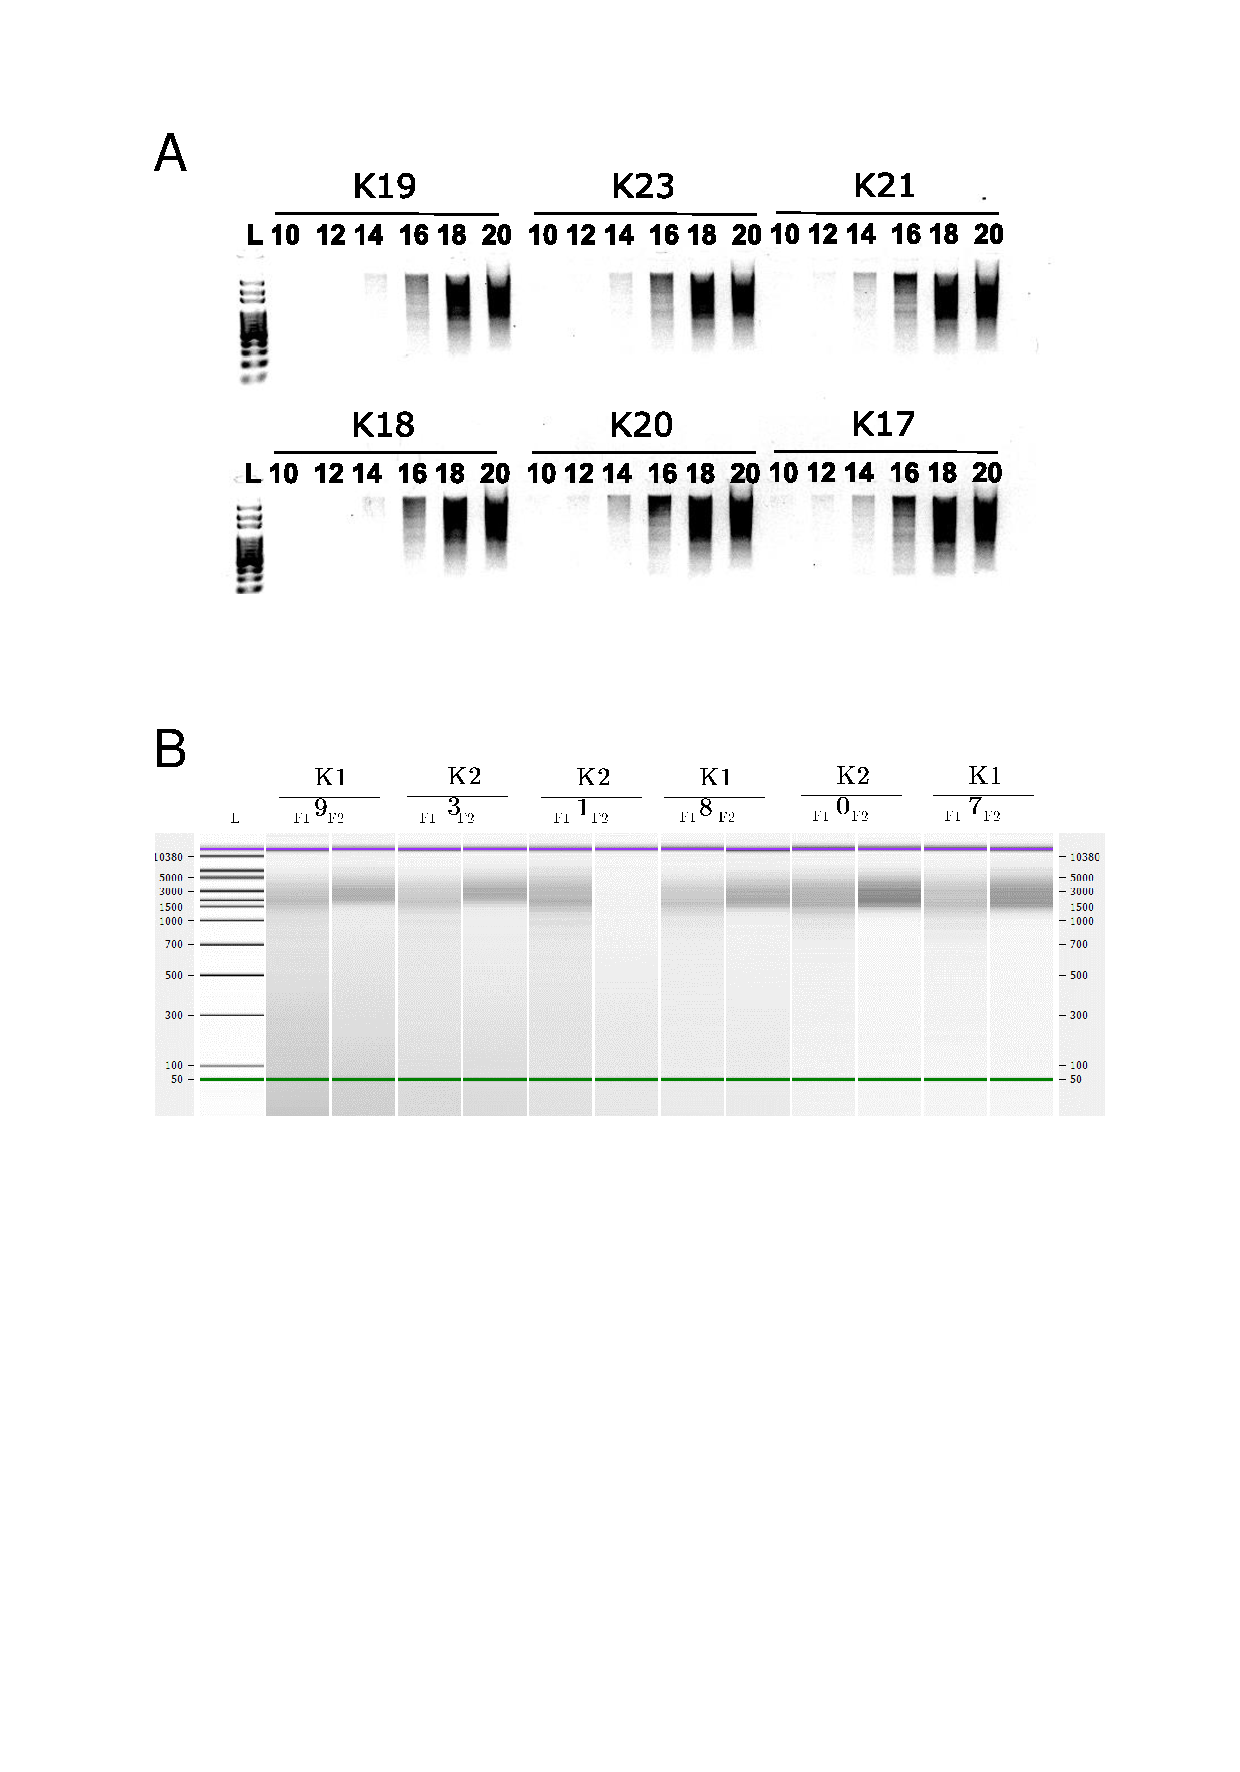
\includegraphics[page=1,trim={0 10cm 0 0cm},clip,scale = 0.75]{Figures/TargetedTranscriptome_ppt.pdf}
	\captionsetup{width=0.95\textwidth}
	\caption[Iso-Seq Targeted Transcriptome - cDNA amplification and purification]%
	{\textbf{The first stage between the targeted and whole transcriptome sequencing is the same with samples typically amplified using 14 cycles followed by enrichment of high molecular weight cDNA in Fraction 2: a)} Like whole transcriptome sequencing, samples were amplified using 14 cycles (Figure \ref{fig:isoseq_whole_pccresults}) whereby cycles below generated insufficient cDNA and cycles above showed signs of over-amplification. The samples shown here (K19, K23, K21, K18, K20, K17) were multiplexed and sequenced in Batch 1 (see Table \ref{tab:mouse_samples_sequenced}. Ladder (L) shown is 100bp DNA ladder. \textbf{B)} Similar to whole transcriptome sequencing, amplified cDNA was further divided into two fractions (denoted here as F1 and F2) and purified with 1X (F1) and 0.4X (F2) AMPure beads. As shown in the Bioanalyzer gel, there was an enrichment of higher-molecular weight cDNA in Fraction 2 compared to Fraction 1 across all the samples (with the exception of Sample K21 with loss of Fraction 2). Green and purple line represent the lower marker at 50bp and the upper marker at 17kb respectively. F1 - Fraction 1 containing cDNA purified with 1X AMPure beads; F2 - Fraction 2 containing cDNA purified with 0.4X AMPure beads.}
	\label{fig:isoseq_targeted_pccresults}
\end{figure}


\begin{figure}[!htp]
	\centering
	\vspace{20pt}
	\includegraphics[page=2,trim={0 8cm 0cm 1cm},clip,scale = 0.75]{Figures/TargetedTranscriptome_ppt.pdf}
	\captionsetup{width=0.95\textwidth}
	\caption[Iso-Seq Targeted Transcriptome - Target Capture and library preparation]%
	{\textbf{Successful target capture and library preparation across all batches, as shown by enrichment of transcripts with specific lengths:} \textbf{A)} and \textbf{c)} are Bioanalyzer electropherogram traces of Batch 1 (n = 6) and Batch 2 (n = 9) respectively after enrichment of cDNA with selective IDT probes ( \cref{section:ch2_targetcapture_explanation}). \textbf{B)}, \textbf{d)} and \textbf{f)} are Bioanalyzer electropherogram traces of Batch 1, 2 and 3 respectively after library preparation (denoted here as "Final", \cref{section:ch2_smrtbelltemplate_explanation}. \textbf{e)} An overlay of Batch 2 after target capture and library preparation. 
	\\
	\\
	As can be seen across all figures, target capture appears to be successful with detected peaks, reflecting enrichment of target transcripts with specific lengths, which differs from the broad peaks that are evident in whole transcriptome sequencing (Figure \ref{fig:isoseq_whole_bioresults}). Library preparation with ligation of SMRT bell templates retained these targeted transcripts with good peak overlay, as seen in figure e). The difference in peak height (i.e. cDNA quantity) between target capture and library preparation is due to a difference in input cDNA concentration when running Bioanalyzer - input cDNA after library preparation was diluted with a 1:5 dilution factor to maximise amount of cDNA available for sequencing, whereas input cDNA after target capture was not diluted.}  
	\label{fig:isoseq_targeted_libresults}
\end{figure}

\begin{figure}[!htp]
	\centering
	\vspace{20pt}
	\includegraphics[page=3,trim={0 18cm 0cm 0cm},clip,scale = 0.75]{Figures/TargetedTranscriptome_ppt.pdf}
	\captionsetup{width=0.95\textwidth}
	\caption[ONT Targeted Transcriptome - Target Capture and library preparation]%
	{\textbf{Successful target capture and ONT library preparation, as shown by enrichment of transcripts with specific lengths:} Shown in \textbf{A)} is the gel snapshot image from the TapeStation Assay of Batch 2 (n = 9) and Batch 3 (n = 9) respectively after enrichment of cDNA with selective IDT probes (\cref{section:ch2_targetcapture_explanation}) and ONT library preparation (\cref{sec: ONTlib_preparation}), and \textbf{B)} is the respective electropherogram of Batch 3. 
	\\
	\\
	Similar to the Bioanalyzer electropherogram from \cref{fig:isoseq_targeted_libresults}, target capture and ONT library preparation appears to be successful with detected peaks, reflecting enrichment of target transcripts with specific lengths. Diluted DNA (1:5 dilution factor) was used for TapeStation Assay to maximise the amount of cDNA available for sequencing. L - Ladder, B2 - Batch 2, B3 - Batch 3. Of note, the ladder used was expired and thus missing the lower green marker. }  
	\label{fig:ONT_targeted_libresults}
\end{figure}


\subsection{ONT Library Preparation and Nanopore Sequencing}
RNA from a subset of mouse samples (n = 2) was prepared for ONT cDNA library preparation and nanopore sequencing using the ONT lab workflow, as detailed and described in \cref{chap:ont_labpipeline}. Briefly, cDNA was similarly prepared from 200ng RNA using the SMARTer PCR cDNA Synthesis Kit (Clontech, UK) (described in \cref{section:ch2_cDNA_synthesis_explanation}), with addition of ERCC standards, followed by PCR amplification of 14 cycles with PrimeSTAR GXL DNA Polymerase (Clontech, UK) (described in \cref{section:ch2_PCR_explanation}). Quantification and size distribution were then determined using Qubit DNA High sensitivity assay (Invitrogen) and Bioanalyzer 2100 (Agilent), and library preparation was proceeded with ONT’s Ligation Sequencing kit (SQK-LSK109) (detailed in \cref{sec: ONTlib_preparation}). Sequencing was then performed on ONT MinION using a FLO-Min106D flow cell (detailed in \cref{sec: ONTlib_sequencing}). 

\subsection{ONT QC and data processing}
QC of raw reads was performed using PycoQC, with subsequent analysis using the ONT bioinformatics pipeline (details are provided in \cref{section:ont_bioinformatics}). Briefly, raw reads were basecalled using \textit{Guppy} (v4.0) and reads with Phred (Q) < 7 filtered out. Primers and ONT adapters were then removed using \textit{Porechop} to generate full-length reads, followed by trimming of polyA tails with \textit{Cutadapt}. Full-length reads were then mapped to the reference mouse genome using \textit{Minimap2} (v2.17) with the following parameters "-ax splice". Owing to the high error rate attributed to ONT sequencing, artifactual noncanonical splice junctions from aligned reads were corrected with \textit{Transcript Clean} and corrected reads were subsequently processed using \textit{TALON} for annotation, quantification and filtering for intrapriming (--maxFracA = 0.5). Novel transcripts were only retained if detected with minimum 2 reads in at least 2 samples. 
 
\begin{figure}[htp]
	\centering
	\includegraphics[page=16,trim={0cm 8cm 0cm 0cm},clip,scale = 0.8]{Figures/ProjectDevelopment_Figures}
	\captionsetup{width=0.95\textwidth,singlelinecheck=off}
	\caption[ONT Bioinformatics Pipeline]%
	{\textbf{ONT Bioinformatics Pipeline.} Shown is a detailed bioinformatics pipeline for processing ONT 1D reads from the targeted sequencing experiments, whereby 20 samples were barcoded and sequenced simultaneously on two flow cells (referred as Batch 2 and Batch 3 of the original Iso-Seq Targeted Transcriptome set). Supplementing \cref{fig:ONT_PacBio_bioinformatics}, raw ONT reads from each flow cell were processed and the demultiplexed into the respective samples, which were then processed independently for collapse and transcript quantification. All the samples from both batches were then merged into one complete dataset, while retaining sample-specific transcript expression. 
	}
	\label{fig:ONT_Targeted_bioinformatics}
\end{figure}

\subsection{Comparison of Iso-Seq and Nanopore datasets}
The Iso-Seq targeted dataset (n = 24 samples) was examined with other datasets using \textit{Gffcompare}; such datasets included transcripts identified from whole transcriptome profiling (n = 12 samples) and ONT-derived transcripts from nanopore targeted sequencing (n = 18 samples). For a fairer comparison, Iso-Seq transcripts from whole transcriptome profiling were re-annotated with \textit{SQANTI3} with no splice junction filtering from short-read RNA-Seq data, and only coverage from the same samples were used for the comparison between the whole and targeted Iso-Seq datasets. Conversely, all processed but unfiltered ONT reads were used for a comprehensive comparison between the two technologies with Iso-Seq derived transcripts as reference.   

\subsection{Transcript annotation and Iso-Seq Quantification}
For a comprehensive characterisation of the AD-associated genes enriched in the mouse transcriptome, the Iso-Seq and ONT datasets were merged using \textit{Gffcompare}. In order to retain both filtered ONT-derived transcripts (minimum 2 reads in at least 2 samples) and ONT-derived transcripts that did not pass through filtering but were also detected using the Iso-Seq platform, a custom python script was written to parse the output from \textit{Gffcompare} to identify Iso-Seq and ONT-derived transcripts with a complete exact match (defined by the class code "="), unique filtered ONT-derived and unqique Iso-Seq-derived transcripts. An output file of the abundance was also generated for each transcript and sample, using the counts either provided from \textit{Cupcake} for Iso-Seq-derived-transcripts, \textit{TALON} for ONT-derived-transcripts or the summation of both for transcripts that were commonly detected in both technologies. The merged dataset was then annotated with \textit{SQANTI3} in combination with mouse reference gene annotations (mouse GENCODE, vm22), FANTOM5 CAGE peaks and \textit{STAR}-aligned RNA-Seq junctions, and were classified as either FSM, ISM, NIC, NNC, antisense, fusion, and intergenic (described in \cref{section: sqanti_annotations}). Transcripts classified as ISM with 3'fragment were assumed to be partial 5'RNA degraded products and discarded. ORFs were predicted using the CPAT program (v3.0.2) using all default parameters and transcripts were predicted as protein-coding if the coding potential score was >0.44 for mouse (CPAT recommended parameters)  

\subsection{Characterisation of AS events and transcript visualisation}
To date, current tools for assessing alternative splicing events were developed for short-read RNA-Seq data and fail to capture the connectivity and complexity of long-read-derived isoforms, particularly in targeted profiling of the transcriptome with deep sequencing coverage. A custom python script ("annotate-common-targeted-transcripts.py") was therefore developed to accurately assess the occurrence of alternative splicing events based on splice junction coordinates of transcript exons relative to exons of all known GENCODE transcripts (mm10). Notably, all the reference transcripts were "flattened" to obtain all the coordinates of known exons. Common alternative splicing events such as alternative first exons (AF), alternative last exons (AL), alternative 5' splice sites (A5), alternative 3' splice sites (A3), intron retention (IR) and exon skipping were assessed. Furthermore, other regulatory mechanisms such as alternative transcription initiation defined by alternative promoter/TSS, alternative termination likewise defined by alternative TTS, and presence of novel exons were evaluated using this custom script.

Alternative 5' and 3' splice sites were defined as splice sites differing by more than 10bp from the known splice site, and an intron was considered retained if the exon splice site differed by more than 100bp from the known splice site. Isoforms were visualised using UCSC genome browser, and were grouped by their splicing patterns to ease visualisation based on the following rank prioritisation: i) all exons with exact splice junction coordinates to know exons, ii) alternative first exons, iii) contain novel exons upstream of first exon, iv) novel exons downstream of last exon, v) characterised with intron retention, exon skipping and novel exons, vi) IR and ES, vii) novel exons within known exons, viii) IR only, ix) ES only and x) all exons with alternative 5' and 3' sites.

%ISM isoforms were assumed as partial products of longer FSM isoforms, and associated read counts were aggregated.  

\begin{figure}[htp]
	\centering
	\includegraphics[page=5,trim={0.5cm 7cm 0cm 0cm},clip,scale = 0.8]{Figures/TargetedTranscriptome_LabResults}
	\captionsetup{width=0.95\textwidth,singlelinecheck=off}
	\caption[Bioinformatics Pipeline for merging targeted Iso-Seq and ONT datasets]%
	{\textbf{Bioinformatics Pipeline for merging targeted Iso-Seq and ONT datasets}. Shown is a outline of the bioinformatics pipeline for processing Iso-Seq reads and ONT reads 1D reads from the targeted transcriptome profiling of the mouse cortex. 
	}
	\label{fig:Targeted_bioinformatics_pipeline}
\end{figure}

\begin{figure}[htp]
	\centering
	\includegraphics[page=7,trim={0cm 1cm 0cm 0cm},clip,scale = 0.8]{Figures/TargetedTranscriptome_LabResults}
	\captionsetup{width=0.95\textwidth,singlelinecheck=off}
	\caption[Characterisation of isoforms detected in targeted transcriptome profiling]%
	{\textbf{Characterisation of isoforms detected in targeted transcriptome profiling}. 
	}
	\label{fig:Targeted_isoforms_annotate}
\end{figure}

\begin{figure}[htp]
	\centering
	\includegraphics[page=8,trim={0cm 1cm 0cm 0cm},clip,scale = 0.8]{Figures/TargetedTranscriptome_LabResults}
	\captionsetup{width=0.95\textwidth,singlelinecheck=off}
	\caption[Determining coding and NMD status]%
	{\textbf{Determining coding and NMD status}.  
	}
	\label{fig:Targeted_isoforms_cpat}
\end{figure}

\newpage
\section{Results}
\subsection{Iso-Seq Run performance and sequencing metrics}
Following Iso-Seq library preparation and SMRT sequencing, a total of XXGb (s.d = XXGb) were obtained (Table \ref{tab:targeted_mouse_run_output}). Of note, 6 samples were first trialled and multiplexed in Batch 1 to determine the yield output and coverage depth - PacBio recommends starting with 4 - 8 samples for multiplexing. Having noticed that an average yield output (24Gb) with a high off-target sequencing, implicating saturation of target genes with 6 samples, the number was increased to 9 samples in Batch 2 and Batch 3. Despite more samples, the sequencing run for Batch 2 and 3, performed by Exeter's Seqeuncing Service, had a poor loading rate (38.1\% P1 of Batch 3 vs 71\% of Batch 1) and low subsequent yield. The samples were also potentially degraded after having been stored in -20\textdegree C for over 6 months due to Covid-19 lockdown. 

The yield difference between the first and last two batches was evident in the number of CCS reads (total = 996K; Batch 1 = 469K, Batch 2 = 306K, Batch 3 = 2221K Figure \ref{fig:isoseq_targeted_run_output}a) and FLNC reads (total = 930K; Batch 1 = 399K, Batch 2 = 275K, Batch 3 = 256K, Figure \ref{fig:isoseq_targeted_run_output}a) generated, after applying the bioinformatics Iso-Seq pipeline (same as the whole transcriptome approach with the exception of removing barcodes rather than general primers). However, calculation of the on-target rate suggested that while Batch 2 and 3 had lower output yield, the coverage of target genes was significantly greater than Batch 1 due to the increased sample size (mean rate in Batch 1 = 34.5\%; mean rate in Batch 2 = 46.2\%; mean rate in Batch 3: 42.9\%, Figure \ref{fig:isoseq_targeted_rate}). The on-target rate is defined as the proportion of mapped transcripts with sequences overlapping at least one target probe. 
%Off-target 

In addition to batch variability, the number of full-length transcripts obtained per sample varied within each batch (Figure \ref{fig:isoseq_targeted_run_output}b). This variability was not associated with RIN (corr = 0.147, P = 0.492, Spearman's rank) and is unlikely to be due to library preparation, given that samples were pooled in equal molarity during target capture. However, there was no significant difference in the number of full-length transcripts between WT and TG across the batched runs (Wilcoxon rank sum test, W = 73, P = 0.977, Figure \ref{fig:isoseq_targeted_run_output}c). 


\begin{table}[]
	\captionsetup{width=1.0\textwidth}
	\caption[Run Yield Output from Targeted Transcriptome Iso-Seq of Tg4510]%
	{Iso-Seq run yield for each batch of Tg4510 mouse samples sequenced using targeted transcriptome approach}
	\label{tab:targeted_mouse_run_output}
	\centering
	\begin{tabularx}{\textwidth}{cccccccccc}
		\toprule
		\multirow{3}{*}{Sample} &
		\multirow{3}{*}{\begin{tabular}[c]{@{}c@{}}Total \\ Bases\\ (GB)\end{tabular}} &
		\multirow{3}{*}{\begin{tabular}[c]{@{}c@{}}Polymerase\\  Reads\end{tabular}} &
		\multicolumn{4}{c}{Read  Length (kB)} &
		\multicolumn{3}{c}{Productivity} \\ \cmidrule(l){4-10} 
		&&&
		\multicolumn{2}{c}{Polymerase} &
		\multicolumn{2}{c}{Subread} &
		\multirow{2}{*}{P0} &
		\multirow{2}{*}{P1} &
		\multirow{2}{*}{P2} \\
		&&&
		Mean & N50 & Mean & N50 &&&
		\\ \midrule
		Batch 1 & 24.2 & 712250 & 34.0 & 70.5 &	1.4 & 1.85 &
		\begin{tabular}[c]{@{}c@{}}4.62\% \\ (46613)\end{tabular} &
		\begin{tabular}[c]{@{}c@{}}71.58\% \\ (722026)\end{tabular} &
		\begin{tabular}[c]{@{}c@{}}24.76\% \\ (249707)\end{tabular} \\
		Batch 2 &
		&&&&&&&
		&
		\\
		Batch 3 &	19.3 &	383292 &	50.5 &	100 &	1.6 &
		2.02 &
		\begin{tabular}[c]{@{}c@{}}18.68\% \\ (189549)\end{tabular} &
		\begin{tabular}[c]{@{}c@{}}38.11\% \\ (386743)\end{tabular} &
		\begin{tabular}[c]{@{}c@{}}43.56\% \\ (442054)\end{tabular} \\ \bottomrule
	\end{tabularx}

	\vspace{1cm}
	\centering
	\begin{tabularx}{\textwidth}{cccccccc}
		\hline
		\multirow{3}{*}{Sample} & \multicolumn{4}{c}{Control}  & \multirow{3}{*}{\begin{tabular}[c]{@{}c@{}}Local\\ Base\\ Rate\end{tabular}} & \multicolumn{2}{c}{Template} \\ \cline{2-5} \cline{7-8} 
		&
		\multirow{2}{*}{\begin{tabular}[c]{@{}c@{}}Total\\  Reads\end{tabular}} &
		\multirow{2}{*}{\begin{tabular}[c]{@{}c@{}}Read \\  Length Mean\end{tabular}} &
		\multicolumn{2}{c}{Concordance} &
		&
		\multirow{2}{*}{\begin{tabular}[c]{@{}c@{}}Adapter\\ Dimer (0-10bp)\end{tabular}} &
		\multirow{2}{*}{\begin{tabular}[c]{@{}c@{}}Short Insert\\ (11- 100bp)\end{tabular}} \\
		&       &        & Mean & Mode &                                                                              &               &              \\ \hline
		Batch 1                 & 9,690 & 31,505 & 0.84 & 0.87 & 2.31                                                                         & 0             & 0            \\
		Batch 2                 &       &        &      &      &                                                                              &               &              \\
		Batch 3                 & 3,440 & 52,533 & 0.85 & 0.87 & 2.86                                                                         & 0             & 0            \\ \hline
	\end{tabularx}
\end{table}


\begin{figure}[!htp]
	\begin{center}
		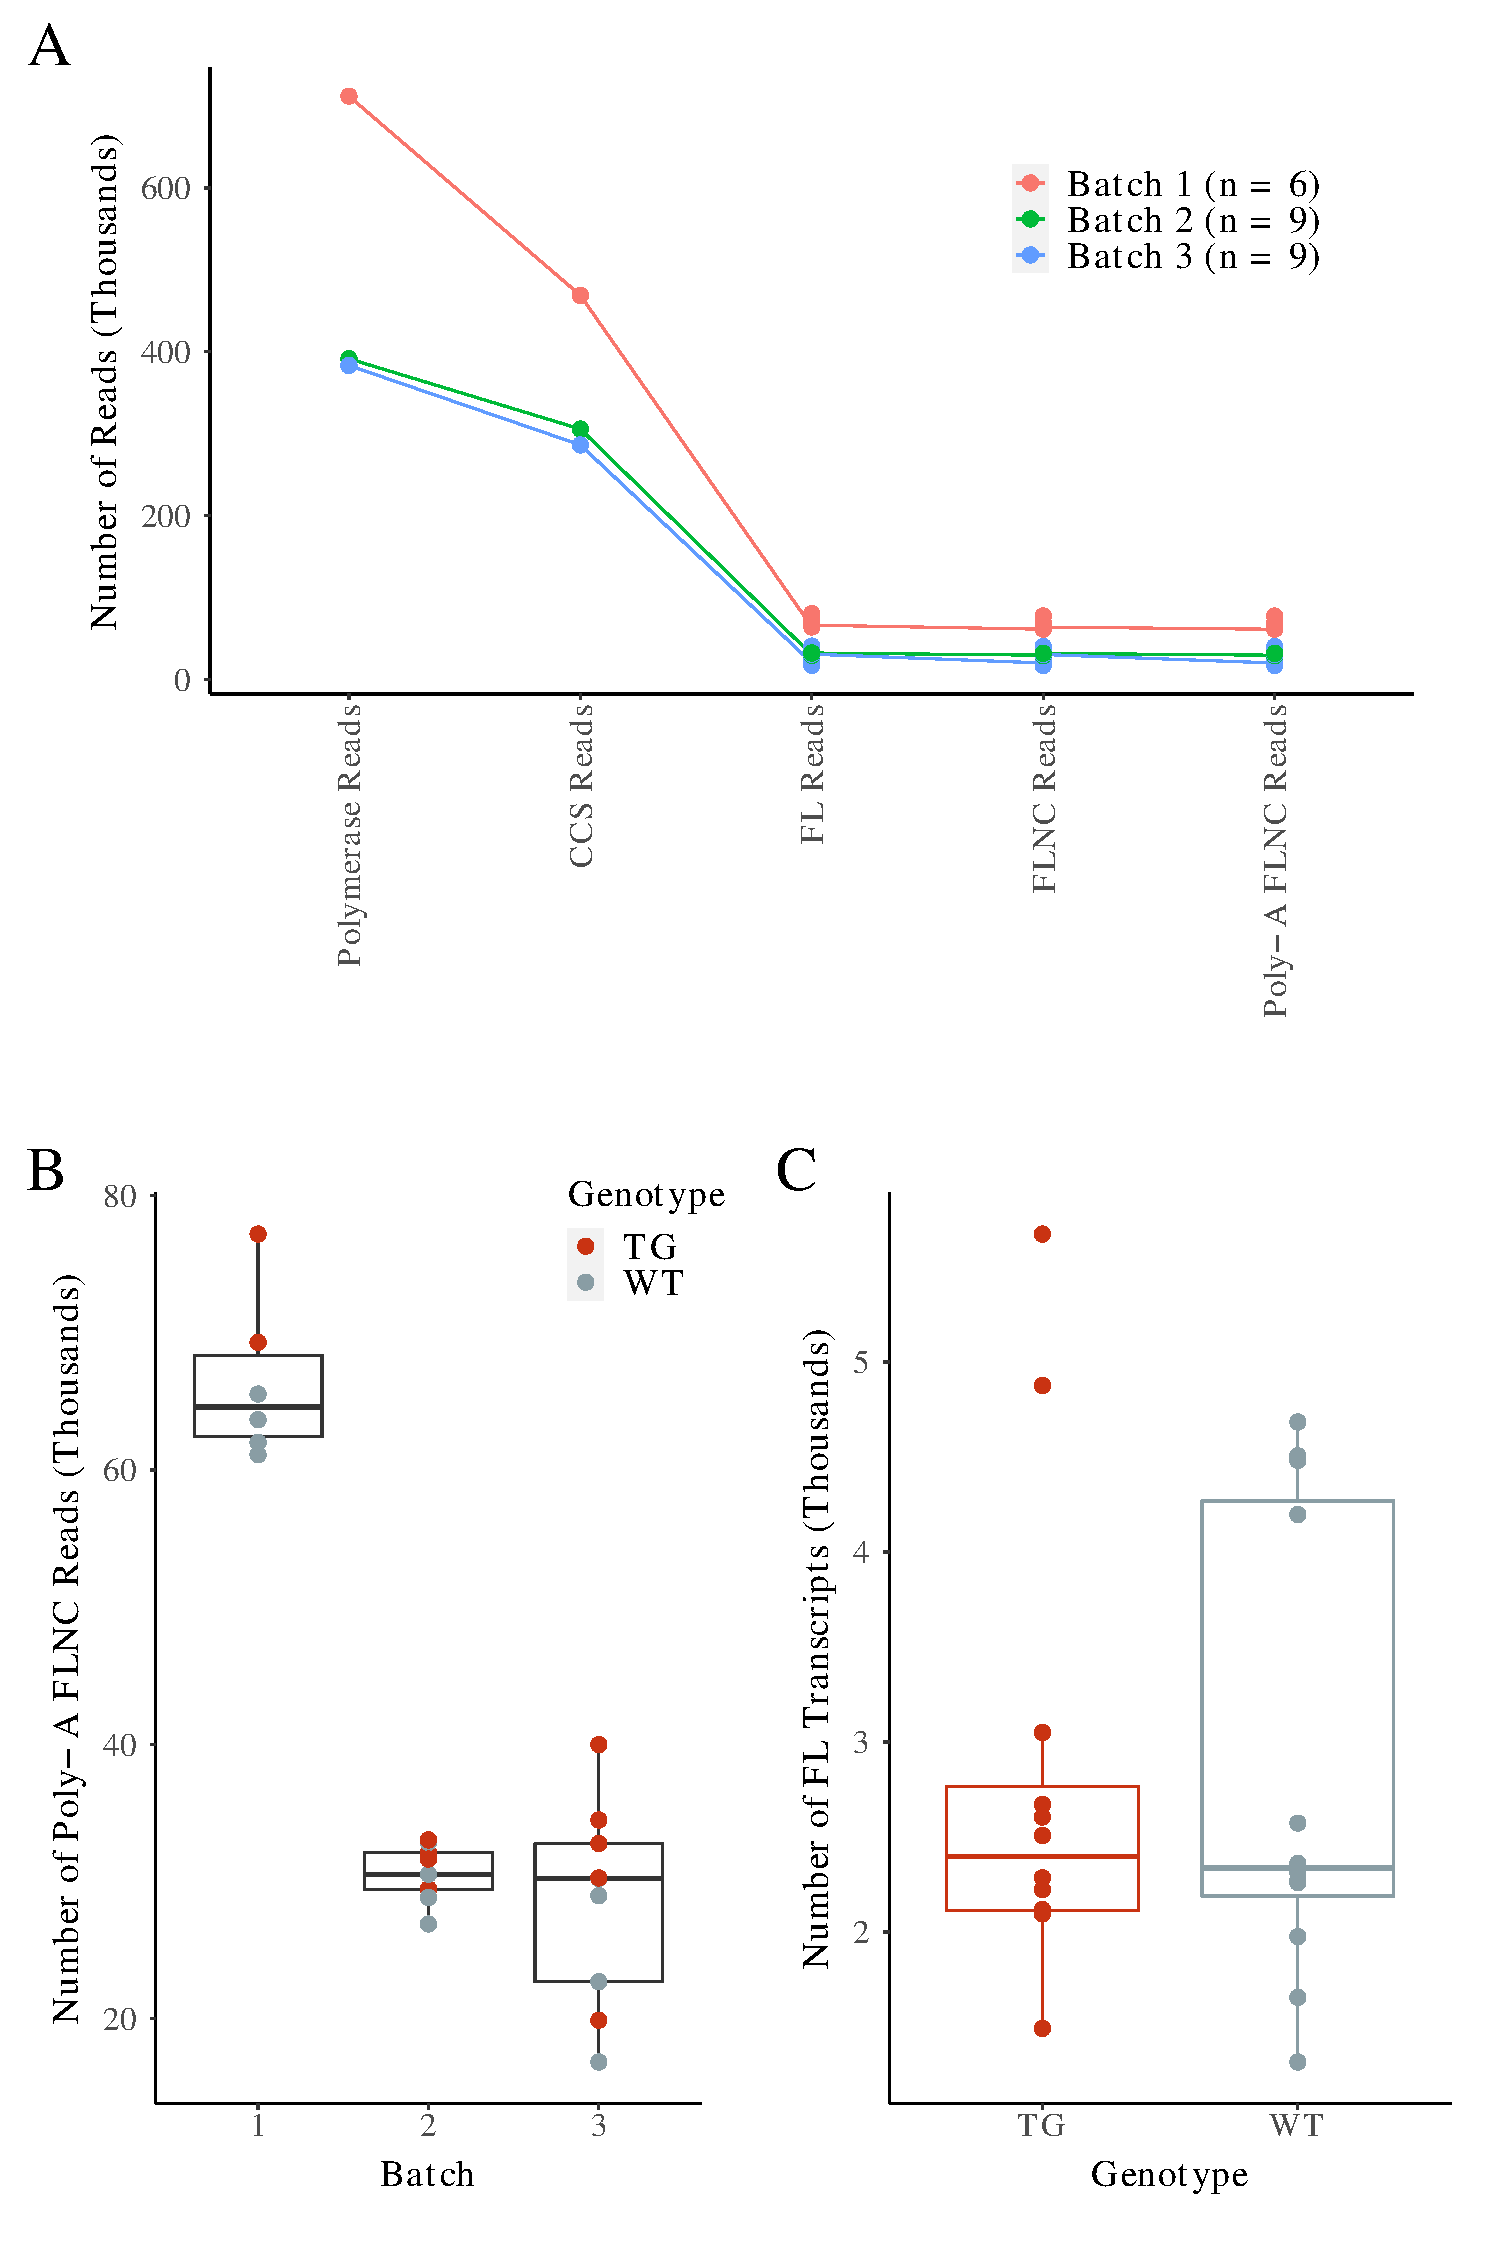
\includegraphics[page=1,trim={0 1cm 0 0},clip,scale = 0.55]{Figures/TargetedTranscriptome.pdf}
	\end{center}
	\captionsetup{width=0.95\textwidth}
	\caption[Targeted Transcriptome Iso-seq run performance]%
	{\textbf{Despite batch variability in targeted transcriptome sequencing, no difference in the number of full-length transcripts was observed between wildtype and transgenic mice}. \textbf{A)} Samples (n = 24) were multiplexed and sequenced in three runs (Batch 1, 2 and 3) with varied performance, as indicated by the number of polymerase reads through to poly-A FLNC reads. In the bioinformatics pipeline, the samples were demultiplexed and individually processed after generation of CCS reads from each run. \textbf{B)} Sample variability within each batch was observed from the number of poly-A FLNC reads generated. However, \textbf{c)} no statistical difference was observed in the overall number of full-length transcripts detected between wild-type and transgenic. Full-length transcripts were collapsed from poly-A FLNC reads in Iso-Seq Cluster. CCS - Circular Consensus Sequence, FLNC - Full-Length Non-Concatemer, FL - Full-Length, WT - Wild-type, TG - Transgenic}
	\label{fig:isoseq_targeted_run_output}
\end{figure}

\begin{figure}[!htp]
	\begin{center}
		\includegraphics[page=2,trim={0 25cm 0 0},clip,scale = 0.55]{Figures/TargetedTranscriptome.pdf}
	\end{center}
	\captionsetup{width=0.95\textwidth}
	\caption[On-Target rate in Transcriptome Iso-Seq runs]%
	{\textbf{Coverage of target genes was greater in Batch 2 and 3 than Batch 1 due to more samples multiplexed and sequenced}. Samples (n = 24) were multiplexed and sequenced in three runs (Batch 1 = 6 samples, Batch 2 = 9 samples, Batch 3 = 9 samples). Despite lower run yield output (\ref{tab:targeted_mouse_run_output}), Batch 2 and Batch 3 had a higher on-target rate, which refers to the proportion full-length transcripts associated with target genes. A difference in the on-target rate between wild-type and transgenic samples was observed in Batch 1, which is a likely reflection of the sample variability in sequencing (Figure \ref{fig:isoseq_targeted_run_output}b). WT - Wild-type, TG - Transgenic}
	\label{fig:isoseq_targeted_rate}
\end{figure}


\subsection{ONT Run performance and sequencing metrics}
Following library preparation and nanopore sequencing on a subset of samples, a total of 28.54M reads (39.68Gb) were generated across two flow cells and a total of 22.8M (80\%) reads were successfully basecalled using \textit{Guppy} (\cref{tab:ont_targetedrun_output}). Despite similar amount of loading onto the flow cell (Batch 2: 540ng, Batch 3: 500ng), there was a large yield difference in the number of basecalled reads between the two batches with Batch 3 generating significantly more reads (Batch 2: 12.3M and Batch 3: 16.3M), and after filtering for read quality (Phred Score > Q7, referring to a read accuracy > 80\%) of which the majority reads passed (Batch 2: 9.68 (78.8\%); Batch 3: 13.13M (99.3\%) (\cref{fig:ONT_targeted_run_output}\textbf{a}). 

Similar to Iso-Seq Targeted Transcriptome run performance, the number of filtered reads obtained per sample varied within each batch (\cref{fig:ONT_targeted_run_output}\textbf{B}), with more reads generated in the transgenic mice in both Batches 2 and 3 (\cref{fig:ONT_targeted_run_output}\textbf{c}, Batch 2: Wilcoxon rank sum test, W = 18, P = 0.063; Batch 3: Wilcoxon rank sum test, W = 17, P = 0.11). This variability was not associated with RIN (corr = -0.267, P = 0.284, Spearman's rank) or barcode (corr = -0.058, P = 0.819, Spearman's rank), but simply a reflection of more transgenic mice sequenced (Batch 2: WT = 4, TG = 5 samples; Batch 3: WT = 4, TG = 5 samples). The difference in number of WT and TG mice in Batches 2 and 3 would have been compensated in Iso-Seq with Batch 1, where there is more WT mice; however, Batch 1 was not sequenced using ONT due to the lack of remaining cDNA. Of note, the difference in the number of reads between TG and WT, while different, was not statistically significant at the 5\% level (Wilcoxon rank sum test, W = 59, P = 0.10, \cref{fig:ONT_targeted_run_output}\textbf{d}).
  
While the throughput was comparable between Iso-Seq and ONT nanopore sequencing for the targeted transcriptome profiling (Iso-Seq: 19.3 - 24.2Gb, ONT: 16.9 - 22.8Gb), ONT nanopore sequencing generated significantly more (1D) reads (12.3M - 16.3M) than the polymerase reads from Iso-Seq (0.3M - 0.7M), which is limited by the number of wells available for sequencing (1M ZMWs), and subsequently 20X the number of full-length reads per sample (Iso-Seq mean PolyA-FLNC reads = 38.7K, range = 16.8K - 77.2K; ONT mean basecalled, filtered reads = 918K, range = 667K - 1.32M). This significant difference in read but comparable yield output is due to the multiple sequencing of the same insert in Iso-Seq with the generation of CCS reads, whereas each insert is only sequenced once in ONT nanopore. This significantly higher yield is therefore achieved at the expense of read accuracy, whereby the average read accuracy in ONT nanopore is 90\% (mean Phred Quality = 10; \cref{tab:ont_targetedrun_output)}, \cref{fig:ont_targetedlengthquality}\textbf{a,b}). Of note, the on-target rate observed in both Iso-Seq and ONT nanopore sequencing was similar at $\tilde{50\%}$ (\cref{fig:isoseq_targeted_rate,fig:ont_targeted_rate}), indicating that more samples could have been sequenced.  

\begin{figure}[htp]
	\begin{center}
		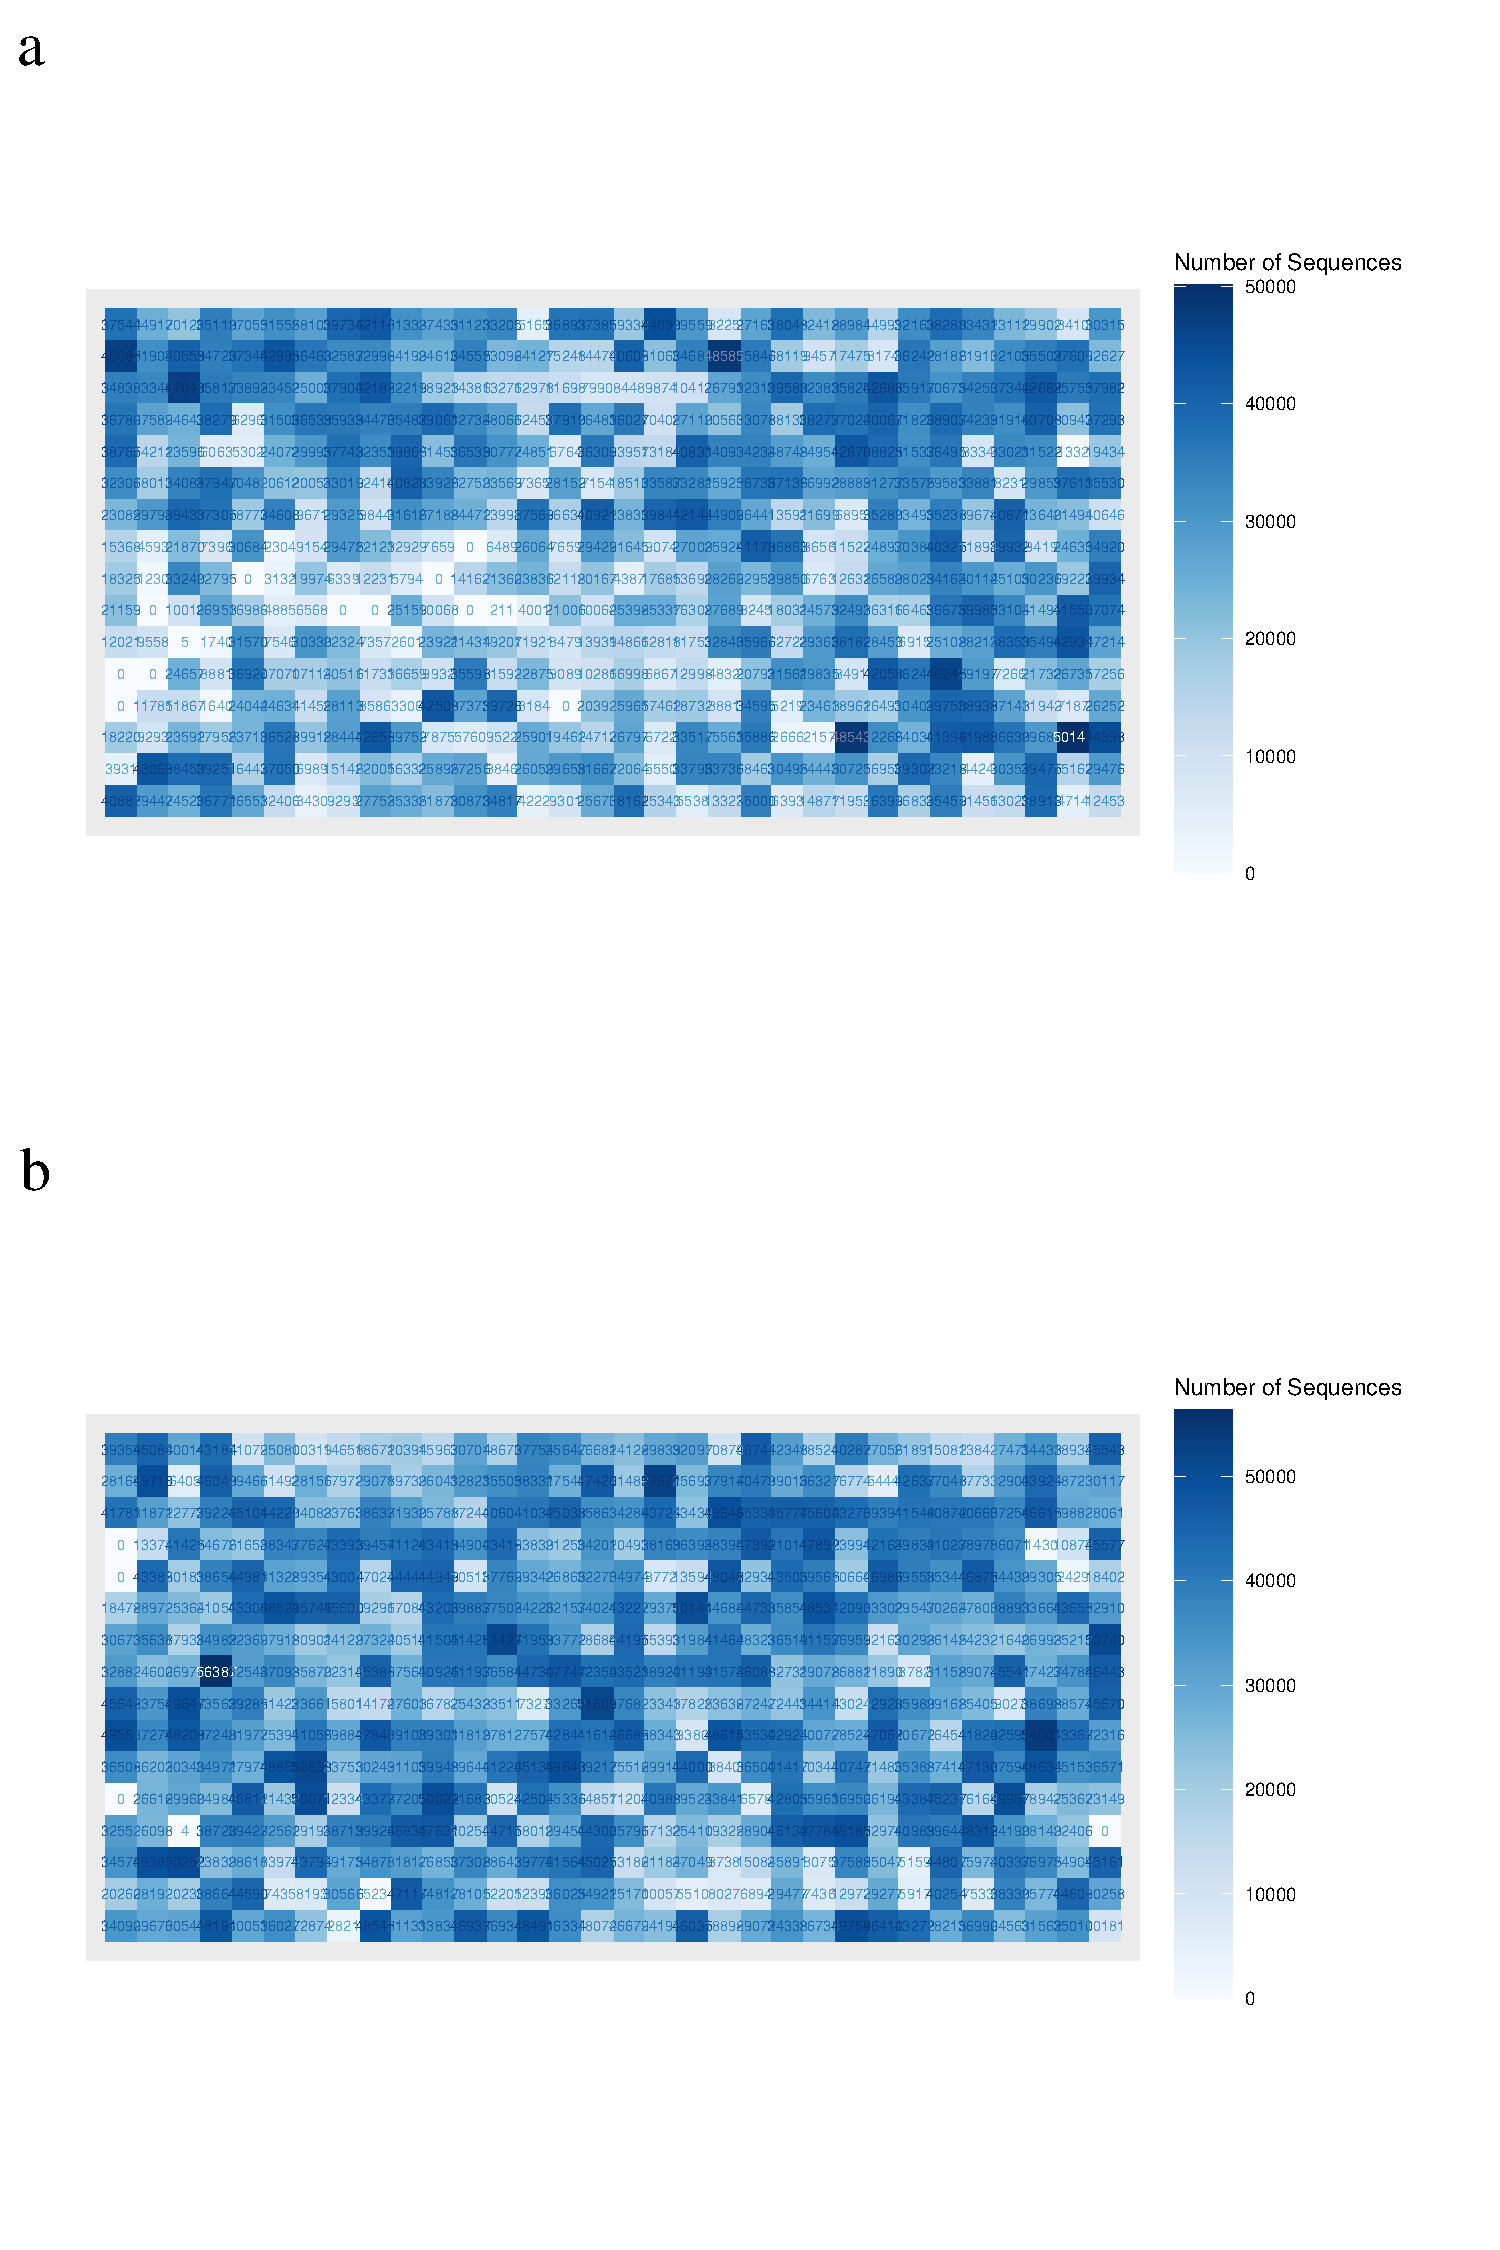
\includegraphics[page=1,trim={0 4cm 0 0},scale = 0.45]{Figures/ONTTargetedTranscriptome.pdf}
	\end{center}
	\captionsetup{width=0.95\textwidth}
	\caption[ONT Sequence Channel Activity from Whole Transcriptome Sequencing ]%
	{\textbf{Sequencing channel activity plot from nanopore sequencing}. Heatmap representation of channel productivity spatially for \textbf{A)} Batch2 (10.1Gb) and \textbf{B)} Batch 3 (3.68Gb) as DNA is translocated through the pore and signal is collected. A contrast of activity can be seen between the two batches, with a number of inactive channels (white box) in Batch 2, and of the channels that are active, fewer DNA molecules are translocated and read.}
	\label{fig:ont_targetedseq_channel}
\end{figure}

%% Qus: Wsa there reflushing?
\begin{figure}[htp]
	\begin{center}
		\includegraphics[page=2,,trim={0 0cm 0cm 10cm},clip, scale = 0.45]{Figures/ONTTargetedTranscriptome.pdf}
	\end{center}
	\captionsetup{width=0.95\textwidth}
	\caption[ONT run performance over time from Whole Transcriptome Sequencing ]%
	{\textbf{Temporal run performance from nanopore sequencing}. Shown is the \textbf{A)} number of basses generated per hour over the course of the sequencing run from Batch 2 and from \textbf{B)} Batch 3, and \textbf{c)} cumulative reads generated from Batch2 and from \textbf{d)} Batch3. The reads are classified as "pass" (dark blue) if QV > 7 and "fail" (light blue) if QV < 7. Gb - Gigabases}
	\label{fig:ont_targetedtime_performance}
\end{figure}


\begin{figure}[!htp]
	\centering
	\includegraphics[page=4,trim={0 0 0 0},clip,scale = 0.55]{Figures/ONTTargetedTranscriptome.pdf}
	\captionsetup{width=0.95\textwidth}
	\caption[ONT Targeted Transcriptome run performance]%
	{\textbf{Significantly more reads were generated in Batch 3 and for transgenic mice in ONT nanopore sequencing}. \textbf{A)} A subset of samples (n = 19) were multiplexed and sequenced in two runs (Batches 2 and 3) with varied performance, as indicated by the number of sequenced reads through to reads demultiplexed per sample. \textbf{B)} Sample variability within each batch not correlated by barcode sequence. \textbf{c)} A reflection of the yield output and sequencing of more transgenic mice, there were more significantly reads generated for transgenic mice individually and \textbf{d)} and across both batches. WT - Wild-type, TG - Transgenic }
	\label{fig:ONT_targeted_run_output}
\end{figure}

\vspace{1cm}
\begin{table}[ht]
	\captionsetup{justification=raggedright,width=0.95\textwidth}
	\caption[Run Yield Output from Targeted Transcriptome Nanopore Sequencing of Tg4510]%
	{\textbf{Comparable run performance and yield output from Targeted Nanopore sequencing of Tg4510}. Two of three batches prepared for targeted transcriptome profiling were also sequenced on ONT MinION on two separate flow cells over 48hours (Batch 2: WT = 4, TG = 5 samples; Batch 3: WT = 4, TG = 5 samples). The number of total reads basecalled was comparable to the targeted sequencing yield with the Iso-Seq approach (\cref{fig:isoseq_targeted_run_output}). Basecalled reads were filtered on quality score with a QV threshold of 7. N50 refers to the sequence length at which 50\% of reads are sized at or over. Gb - Gigabases. Med - Median}
	\label{tab:ont_targetedrun_output}
	\centering
	\begin{tabularx}{0.95\textwidth}{@{}ccccc@{}}
		\toprule
		\multirow{2}{*}{Sample} & \multicolumn{2}{c}{All Reads}      & \multirow{2}{*}{Active channels} & \multirow{2}{*}{Run Duration} \\ \cmidrule(lr){2-3}
		& Total Bases (Gb) & Number of Reads &                                  &                               \\ \midrule
		Batch 2                     & 16.9             & 12,274,792       & 479                              & 48hours                       \\
		Batch 3                     & 22.8             & 16,274,909       & 425                              & 48hours                       \\ \bottomrule
	\end{tabularx}
	\vspace{1cm}

	\begin{tabularx}{0.95\textwidth}{@{}ccccccccc@{}}
		\toprule
		\multirow{2}{*}{Sample} & \multirow{2}{*}{\begin{tabular}[c]{@{}c@{}}Total Bases\\ (Gb)\end{tabular}} & \multirow{2}{*}{\begin{tabular}[c]{@{}c@{}}Number of\\  Reads\end{tabular}} & \multicolumn{4}{c}{Read Length (bp)} & \multicolumn{2}{c}{Read Quality} \\ \cmidrule(l){4-9} 
		&                                                     &                                                                             & Med  & Mean & N50  & Longest Read & Med           & Mean          \\ \midrule
		Batch 2                     & 14.2                                                                        & \begin{tabular}[c]{@{}c@{}}9,675,186 \\ (78.8\%)\end{tabular}               & XXX   & 1478 & 1779 & 19081        & XXX              & 10.2           \\
		Batch 3                     & 19.41                                                                         & \begin{tabular}[c]{@{}c@{}}13,129,731\\  (80.7\%)\end{tabular}               & XXX    & 1468 & 1813 & 20476        & XXX             & 9.9          \\ \bottomrule
	\end{tabularx}
\end{table}


\begin{figure}[ht]
	\centering
	\includegraphics[page=5,trim={0 27cm 0 0cm},clip,scale = 0.55]{Figures/ONTTargetedTranscriptome.pdf}
	\captionsetup{width=0.95\textwidth}
	\caption[On-Target rate in ONT nanopore runs]%
	{\textbf{Comparable on-target rate in ONT nanopore sequencing to Iso-Seq with a 40-50\% on target rate}. Samples (n = 18) were multiplexed and sequenced in two runs (Batch 2 = 9 samples, Batch 3 = 9 samples). The on-target rate, was similar to that observed in Iso-Seq targeted sequencing (\cref{fig:isoseq_targeted_rate}). A difference in the on-target rate between wild-type and transgenic samples was observed in both batches, a likely reflection of the sample variability in sequencing (\cref{fig:ONT_targeted_run_output}\textbf{c,d}). WT - Wild-type, TG - Transgenic}
	\label{fig:ont_targeted_rate}
\end{figure}

\begin{figure}[htp]
	\begin{center}
		\includegraphics[page=3,trim={0 0cm 0cm 10cm},clip, scale = 0.45]{Figures/ONTTargetedTranscriptome.pdf}
	\end{center}
	\captionsetup{width=0.95\textwidth}
	\caption[ONT read length and quality from Whole Transcriptome Sequencing ]%
	{\textbf{Length and quality distribution of ONT basecalled reads}. Shown are histograms of the number of sequenced reads against \textbf{A)} mean read quality score of Batch 2, \textbf{B)} mean read quality score of Batch 3, and against \textbf{c)} length of Batch 2 and of \textbf{d)} Batch 3. The distribution has been shaded for reads that have passed or failed the quality filter (Q-score threshold of 7). N50 refers to the sequence length at which 50\% of reads are sized at or over. }
	\label{fig:ont_targetedlengthquality}
\end{figure}

\clearpage
\subsection{Iso-Seq Targeted approach detects many more novel transcripts than whole transcriptome profiling}
\label{ch6: wholevstargeted}
% Number of Iso-Seq transcripts
After filtering for technical artefacts (563 (1.69\%) isoforms were removed due to intra-priming, 314 (0.94\%) isoforms were removed due to RT switching, 1,267 (3.80\%) were removed due to likely partial degradation), a total of 4,780 isoforms were detected across 20 AD-associated target genes across all the samples (n = 24). Of these isoforms, an overwhelming majority were novel (n = 4601, 96.2\%) with no RNA-Seq support (n = 24 samples, total number of uniquely mapped reads = 360 million) at the junction (n = 4,033, 84.4\%). This is likely to be reflection of the low coverage of RNA-Seq reads per sample (mean number of uniquely mapped reads = 15 million) to comprehensively span these novel junctions, rather than an indication of the invalidity of these isoforms given the stringent processing of the Iso-Seq bioinformatics pipeline. 

We next wanted to compare the isoform diversity and sequencing coverage of the panel of AD-associated genes captured using the targeted and whole transcriptome approach. As expected, enrichment and selective sequencing of the target genes detected many more transcripts that were not detected in the whole transcriptome approach, the majority of which were novel (NIC: XX, XX\%; NNC: XX, XX\%). Further examination of these transcripts unique to the targeted approach revealed them to be more lowly-expressed than the transcripts detected from both sequencing approaches, highlighting the greater sensitivity of the targeted approach in detecting the novel, rarer transcripts. 

Conversely with a target rate of \textasciitilde{XX\%}, the targeted sequencing experiments detected many isoforms associated with non-target genes, which were found to be more highly expressed than the isoforms of non-target genes that were uniquely detected in the whole transcriptome approach. This indicates that the off-target genes from the targeted transcriptome are the most abundance rather than based on similar sequence homology to garget genes. 

Intriguingly, the whole transcriptome approach detected isoforms associated with all the target genes with the exception of \textit{Trpa1}, which is the least expressed in the mouse cortex and was only detected in the targeted approach.  Given that we have previously showed that our whole transcriptome Iso-Seq sequencing datasets (n = 12 samples) was close to saturation, we do not anticipate that we would detect \textit{Trpa1} with more samples. This suggests that our sequencing coverage at a total XX Iso-Seq reads were capped at detecting genes above XXTPM.   

\begin{figure}[!htp]
	\begin{center}
		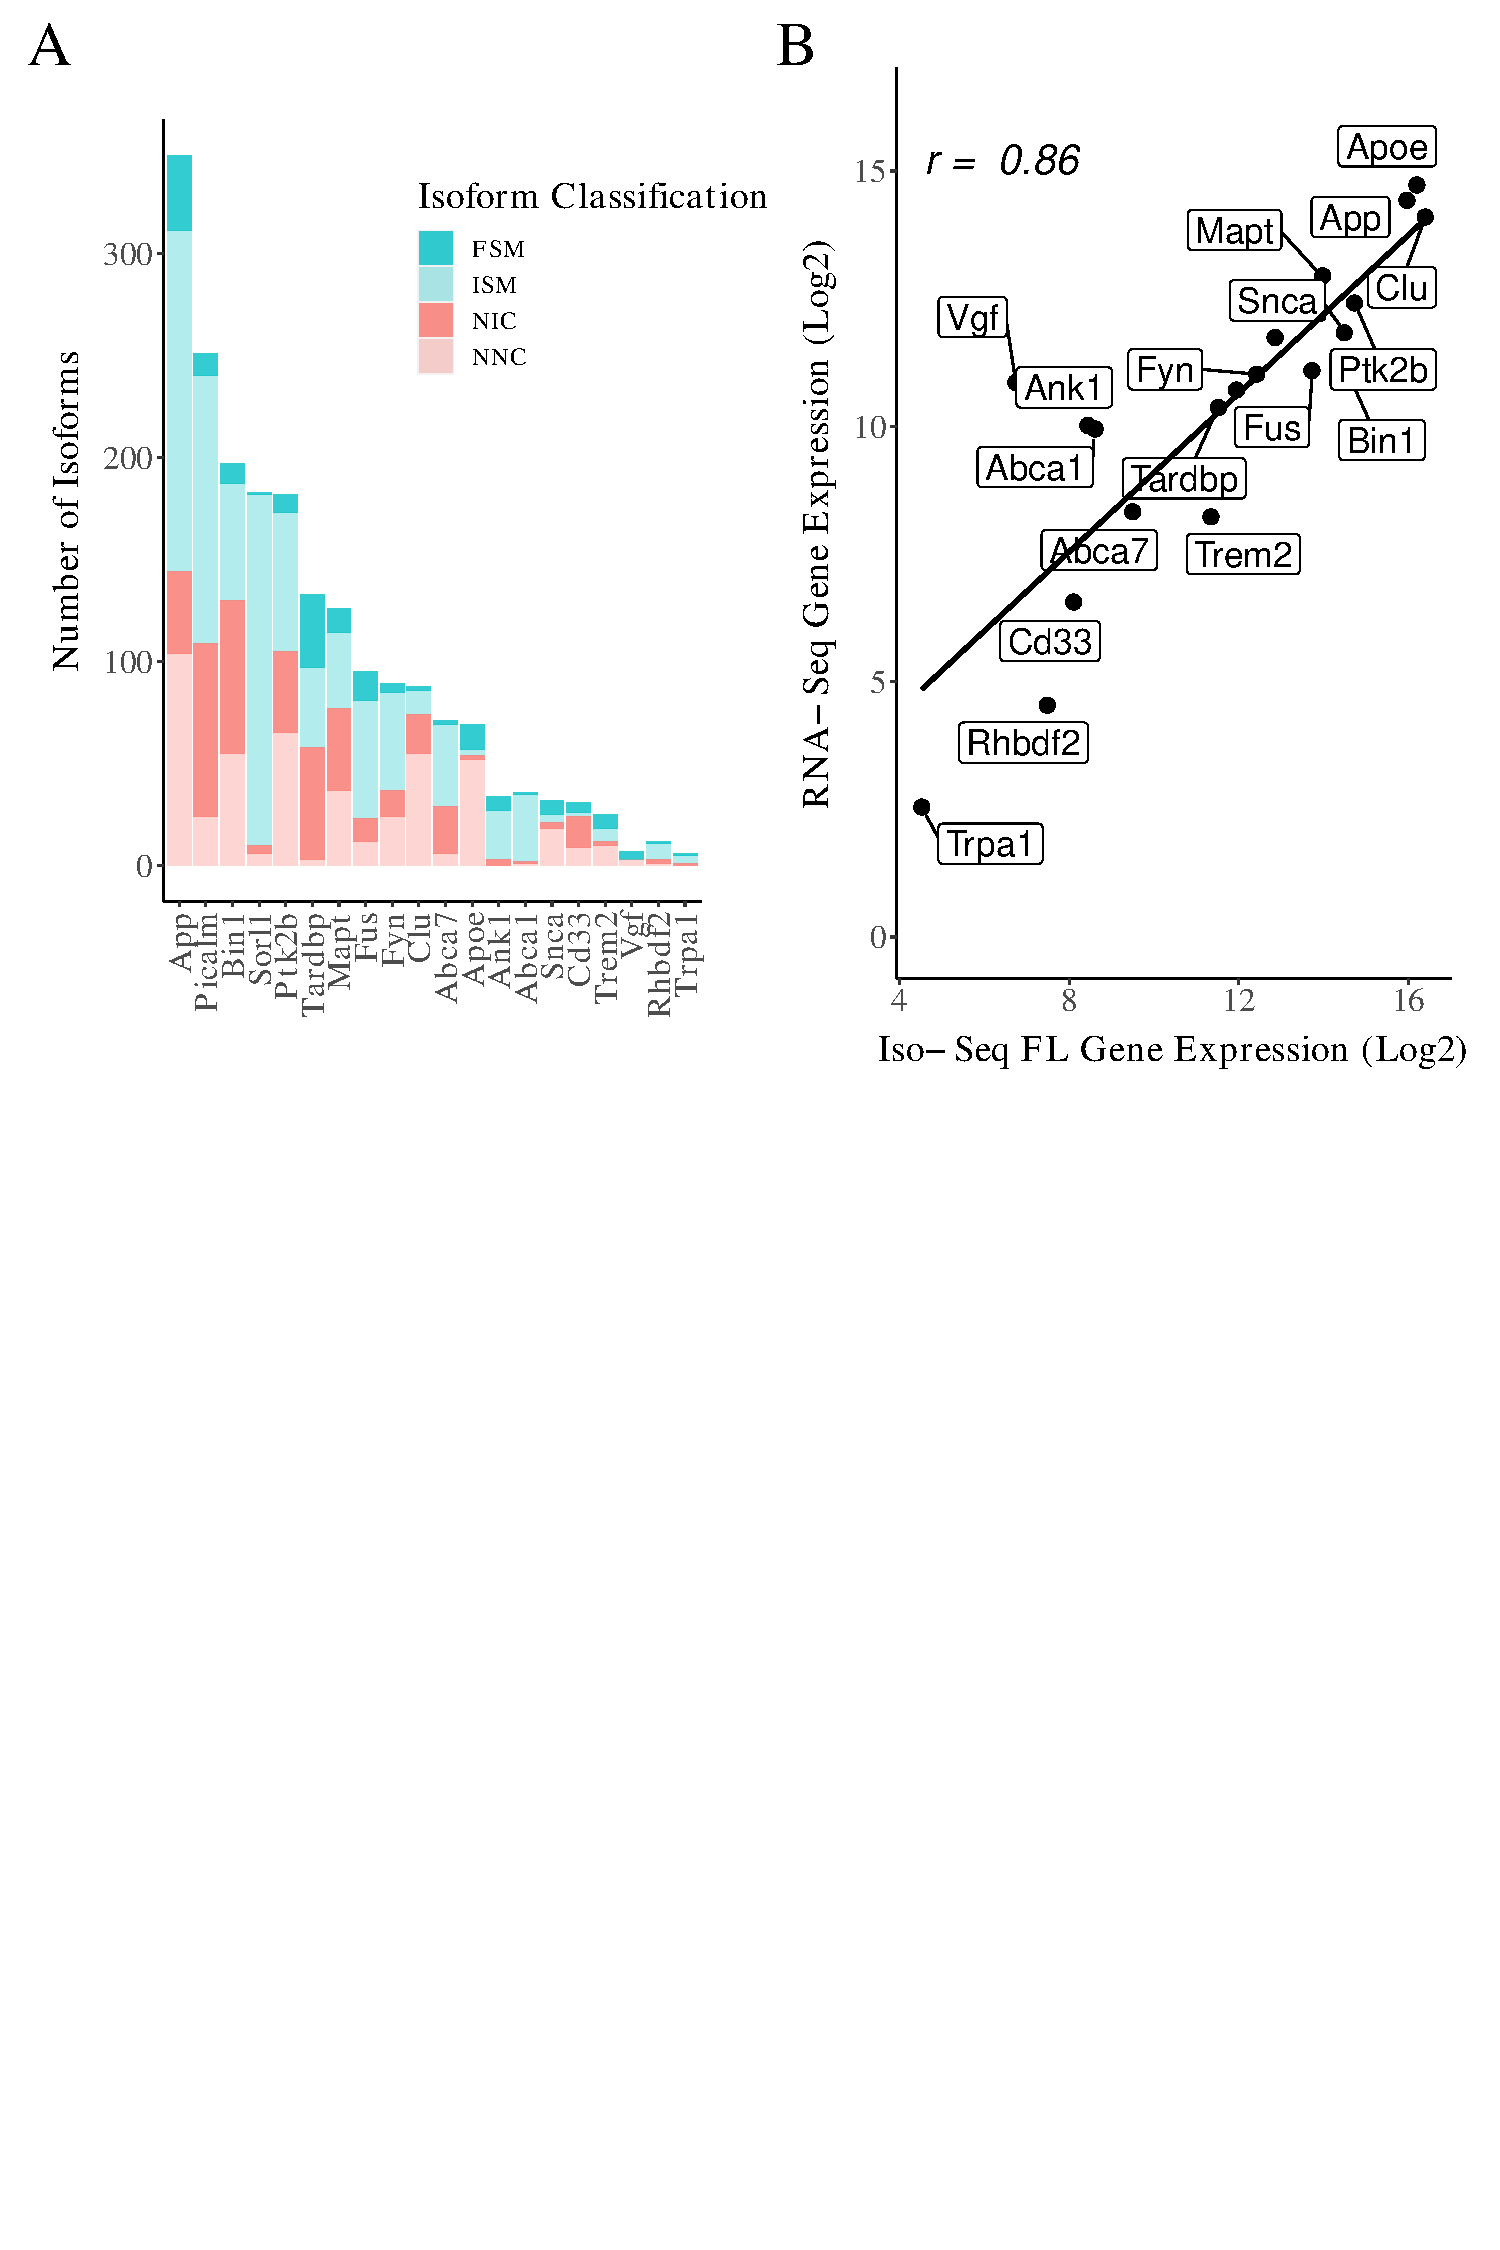
\includegraphics[page=1,trim={0 20cm 0 0cm},clip,scale = 0.60]{Figures/ONTvsIsoSeq.pdf}
	\end{center}
	\captionsetup{width=0.95\textwidth}
	\caption[Wide isoform diversity in AD-associated genes from Targeted Sequencing in mouse cortex]%
	{\textbf{Wide isoform diversity observed in AD-associated genes with many novel isoforms detected}. \textbf{A)} Shown is the number of isoforms detected per target gene from the Iso-Seq targeted dataset, classified by novel and known, after sequential processing and filtering in the bioinformatics Iso-Seq pipeline. Novel isoforms refer to isoforms that are not known in current existing annotations. \textbf{B)} A strong correlation was observed between Iso-Seq and RNA-Seq gene expression. Iso-Seq gene expression was determined from the summation of full-length read counts of associated transcripts, whereas RNA-Seq gene expression was deduced from the normalised \textit{DESeq} counts of aligned RNA-Seq reads to reference genome\cite{Castanho2020}.}
	\label{fig:isoseq_targeted_finalnumberiso}
\end{figure}


\begin{figure}[!htp]
	\begin{center}
		\includegraphics[page=3,trim={0 1.5cm 0 0cm},clip,scale = 0.55]{Figures/TargetedTranscriptome.pdf}
	\end{center}
	\captionsetup{width=0.95\textwidth}
	\caption[Comparison of whole transcriptome vs targeted Iso-Seq transcriptome profiling]%
	{\textbf{Iso-Seq targeted approach detected many more novel and rarer transcripts than whole transcriptome profiling of the mouse cortex}. Shown is the \textbf{A)} number of isoforms per target gene that were uniquely detected using the Iso-Seq targeted approach, uniquely detected in the whole approach and in both datasets, and the \textbf{B)} number of isoforms in the Iso-Seq targeted approach stratified by structural category. \textbf{C)} A box-plot of the full-length read counts of isoforms associated to target and non-target genes from whole transcriptome profiling approach and \textbf{D)} targeted approach. Target genes refer to the panel of 20 AD-associated genes that were enriched for targeted sequencing. FSM - Full Splice Match, ISM - Incomplete Splice Match, NIC - Novel In Catalogue, NNC - Novel Not in Catalogue.}
\end{figure}

\clearpage
\subsection{ONT achieves significantly deeper sequencing coverage than Iso-Seq with enrichment of shorter novel transcripts}
A total of XX transcripts were identified after enrichment of 20 AD-associated genes followed by nanopore sequencing (median = XX, range = XX - XX). Further filtering of novel transcripts by expression (minimum 2 reads in 2 samples) reduced the total number of transcripts by XX fold, suggesting that a vast number of ONT novel transcripts were detected with one FL read and were not reproducibly detected across biological replicates. 

After filtering, we detected a total of XXX isoforms across the same panel of AD-associated genes - XX times more than the Iso-Seq targeted dataset despite sequencing fewer samples (Iso-Seq: n = 24 samples, ONT = 18 samples). Similar to Iso-Seq dataset, target gene expression level was strongly correlated between ONT expression and RNA-Seq expression. However, strikingly the order of the isoform diversity across the panel differed between the two datasets - i.e. \textit{XXX} was associated with the greatest number of transcripts in Iso-Seq whilst \textit{XXX} was the most "isoformic" in ONT dataset, suggesting that some genes were more likely to be sequenced using the ONT platform. Further examination of the two datasets revealed an enrichment of transcripts sized 1-2kb with 5 exons (mean = X, XX) whereas Iso-Seq-derived transcripts were typically longer with more exons (mean = X, XX). This suggests an over-representation of shorter transcripts in the ONT library, a phenomenon that has been previously reported and may be attributed to premature termination of ONT transcript sequencing. 

\begin{figure}[!htp]
	\begin{center}
		\includegraphics[page=2,trim={0 20cm 0 0cm},clip,scale = 0.60]{Figures/ONTvsIsoSeq.pdf}
	\end{center}
	\captionsetup{width=0.95\textwidth}
	\caption[ONT is more sensitive than Iso-Seq with greater power to detect novel transcripts]%
	{\textbf{ONT is more sensitive than Iso-Seq with greater power to detect novel transcripts}. \textbf{A)} Shown is the number of isoforms detected per target gene from the ONT targeted dataset, either classified as known (FSM, ISM) or novel (NIC, NNC), after sequential processing and filtering in the bioinformatics ONT pipeline. Novel isoforms refer to isoforms that are not known in current existing annotations. \textbf{B)} A stronger correlation is observed between ONT gene expression and RNA-Seq gene expression, than Iso-Seq gene expression and RNA-Seq gene expression (\cref{fig:isoseq_targeted_finalnumberiso}\textbf{B}). ONT gene expression is similarly determined from the summation of full-length read counts of associated transcripts, whereas RNA-Seq gene expression was deduced from the normalised \textit{DESeq} counts of aligned RNA-Seq reads to reference genome\cite{Castanho2020}.}
	\label{fig:ont_targeted_finalnumberiso}
\end{figure}

However, significantly more ONT-derived Transcripts were found with TSS annotated with 50bp of a CAGE peak compared to Iso-Seq-derived transcripts, half of which were found over 200bp from the closest annotated CAGE peak. The 5' and 3' ends of ONT-derived transcripts were also more likely to be within 50bp from the closest annotated 5' and 3' ends of the target gene. Perhaps even more telling, a greater proportion of Iso-Seq-derived transcripts were classified as "ISM" (Incomplete Splice Match) with a 3' fragment that matches the 3'end of a known transcript, and are likely to represent truncated products. Furthermore, the majority of ONT-derived transcripts were supported by matched short-read RNA-Seq data (support is defined by all splice junctions supported by more than 1 RNA-Seq read) whereas almost all Iso-Seq-derived transcripts were supported. Notably, a significant difference in number of transcripts supported by RNA-Seq reads was observed with Iso-Seq derived transcripts more likely to be supported - however, we suspect this difference is driven by the greater sensitivity of ONT to detect rare, novel transcripts and relatively insufficient coverage of RNA-Seq reads. Examination of these novel transcripts not supported by RNA-Seq revealed them to be less abundant (median expression = XX FL reads) compared to those supported by RNA-Seq (median expression = XX FL reads).  However, no significant difference in the number of transcripts located to 50bp of CAGE peak was found (Fisher's exact test: XXX), highlighting the power of targeted sequencing for detection of rare, novel isoforms. 

\begin{figure}[!htp]
	\begin{center}
		\includegraphics[page=3,trim={0 0cm 0 0cm},clip,scale = 0.60]{Figures/ONTvsIsoSeq.pdf}
	\end{center}
	\captionsetup{width=0.95\textwidth}
	\caption[Comparison of ONT-derived and Iso-Seq-derived isoforms for targeted transcriptome profiling]%
	{\textbf{While ONT-derived isoforms are generally shorter with fewer exons, the 5' and 3' ends are more within the range of annotated sites and CAGE peaks than Iso-Seq derived isoforms}. \textit{Caption continues on the following page.}}
	\label{fig:ont_isoseq_description}
\end{figure}
\begin{figure}[t]
	\captionsetup{width=0.95\textwidth}
	\contcaption{Shown are density plots of \textbf{A)} the distribution of the transcript lengths and \textbf{B)} exon number in the targeted Iso-Seq (n = 24 samples) and ONT datasets (n = 16 samples). Distance between \textbf{C)} TSS and closest annotated CAGE peak (a negative value refers to a CAGE peak located upstream of TSS), \textbf{E)} TSS and reference TSS (a negative value refers to a query start downstream of reference), \textbf{G} TTS and reference TSS (a negative value refers to a query end upstream of reference).  Proportion of isoforms \textbf{D)} classified within 50bp of a CAGE peak, \textbf{F)} within 50bp of a reference TSS and \textbf{H} within 50bp of a reference TTS. TSS - Transcription start site, TTS - Transcription termination site. Iso-Seq and ONT refer to isoforms from the Iso-Seq and ONT targeted profiling dataset, respectively.}%
\end{figure}

Comparison of the two datasets using \textit{Gffcompare} revealed that the vast majority of Iso-Seq derived transcripts were also detected in ONT nanopore sequencing (n = XX transcripts, XX\%),whereas only a small proportion of filtered ONT-transcripts were detected in Iso-Seq (n = XX transcripts, XX\%). Further examination of these unique ONT-derived transcripts revealed them to be more lowly-expressed and shorter with fewer exons than the commonly-detected ONT-derived transcripts, demonstrating ONT's greater sensitivity at detecting shorter transcripts. In contrast, no difference in length or exon number was observed between the unique and commonly-detected Iso-Seq derived transcripts, suggesting that these are transcripts that were unique to the remaining samples that were not sequenced with ONT. 

Finally, we compared the number of isoforms from the Iso-Seq and ONT datasets against the number of known reference isoforms, the gene length, transcript length (longest known reference isoform) and number of exons. Similar to previous findings, the number of detected isoforms in the Iso-Seq dataset was strongly correlated with gene length and the number of known associated isoforms. However strikingly, a significantly weaker correlation was observed between the number of detected isoforms in the ONT dataset with known isoform number and gene length. Given that far more novel isoforms were detected in ONT dataset with greater sequencing coverage and depth compared to Iso-Seq dataset, this suggests that gene length and number of exons are not the primary driving factors of isoform diversity in this panel of target genes. Indeed, several genes harbour over 25 exons but are only characterised with relatively few exons; examples include \textit{Rhbdf2} with 20 exons and 28 transcripts, \textit{Trpa1} with 27 exons and 11 transcripts, and \textit{Abca1} with 50 exons and 61 transcripts. Conversely, \textit{Apoe} was characterised with the greatest isoform diversity with >5000 transcripts, despite only having 4 exons. 

\begin{figure}[htp]
	\centering
	\vspace{20pt}
	\includegraphics[page=4,trim={0 17cm 0 0cm},clip,scale = 0.75]{Figures/TargetedTranscriptome_ppt.pdf}
	\captionsetup{width=0.95\textwidth}
	\caption[Total number of transcripts detected from Iso-Seq and ONT targeted sequencing]%
	{\textbf{Total number of transcripts detected from Iso-Seq and ONT targeted sequencing}. Shown is a Venn diagram of the total number of AD-associated transcripts (20 target genes) detected in Iso-Seq (shaded red) and ONT (shaded blue) targeted datasets. "ONT filtered" transcripts refer to the subset of ONT transcripts that were retained after \textit{TALON} filtering (minimum 2 reads in at least 2 samples). The green dash refers to the subset of transcripts from ONT and Iso-Seq targeted datasets taken further for downstream annotation and quantification analysis}
	\label{fig:ont_isoseq_venn}
\end{figure}

\begin{figure}[!htp]
	\begin{center}
		\includegraphics[page=4,trim={0 0cm 0 0cm},clip,scale = 0.60]{Figures/ONTvsIsoSeq.pdf}
	\end{center}
	\captionsetup{width=0.95\textwidth}
	\caption[Comparison of the length, expression and exon number of common vs unique isoforms detected from targeted transcriptome profiling]%
	{\textbf{Isoforms detected in both Iso-Seq and ONT targeted dataset are more abundant, and longer with more exons than isoforms unique to ONT dataset}. \textit{Caption continues on the following page.}}
	\label{fig:ontvsisoseq_description}
\end{figure}
\begin{figure}[t]
	\captionsetup{width=0.95\textwidth}
	\contcaption{Shown are box-plots of the \textbf{A)} expression, \textbf{C)} length and \textbf{E)} exon number of transcripts annotated to AD-associated genes (target genes) that were either detected in both Iso-Seq and ONT targeted datasets, or unique to the Iso-Seq (n = 24 samples) and ONT dataset (n = 16 samples). Further shown are correlations of the \textbf{B)} expression, \textbf{D)} length and \textbf{F)} and exon number of the common transcripts that were detected in both datasets. The Iso-Seq and ONT transcript expression refer to the respective full-length read count for the associated isoform.}%
\end{figure}

\begin{figure}[!htp]
	\begin{center}
		\includegraphics[page=5,trim={0 0cm 0 0cm},clip,scale = 0.60]{Figures/ONTvsIsoSeq.pdf}
	\end{center}
	\captionsetup{width=0.95\textwidth}
	\caption[]%
	{\textbf{ }. .}
	\label{fig:commonvsunique_description}
\end{figure}


\begin{table}[!hp]
	\centering
	\captionsetup{width=0.95\textwidth}
	\caption[Relationship between the number of isoforms from targeted datasets and genomic features]%
	{\textbf{Relationship between the number of isoforms from targeted datasets and genomic features}. Shown is a table of the correlation of the number of isoforms from the targeted dataset with the number of reference isoforms, gene length, gene expression, length and exon number of the longest transcript. The merged dataset refer to the subset of transcripts encapsulated by the green dash line in \cref{fig:ont_isoseq_venn}. )}
	\label{tab:isoformnum_corr}	
	\begin{tabular}{cccc}
		\hline
		\multirow{2}{*}{Features} & \multicolumn{3}{c}{Total number of isoforms (AD-associated target genes)} \\ \cline{2-4} 
		& Iso-Seq & ONT & Merged \\ \cline{1-4} 
		Gencode Isoform Number & 0.57 (0.008) & 0.37 (0.109)     & 0.43 (0.061)     \\
		Gene Length            & 0.41 (0.072) & -0.02 (0.938)    & -0.08 (0.745)    \\
		Transcript Length      & 0.3 (0.198)  & -0.4 (0.08314)   & -0.45 (0.046)    \\
		Gene Expression        & 0.68 (0.001) & 0.86 (9.620e-07) & 0.84 (4.416e-06) \\
		Exon Number            & 0.11 (0.643) & -0.4 (0.080)     & -0.51 (0.020)    \\ \hline
	\end{tabular}
\end{table}

\clearpage

\subsection{Characterisation of AS events in AD-associated genes}
The significant deep sequencing coverage achieved with target gene enrichment, particularly with ONT nanopore sequencing, identified hundreds of novel transcripts across the panel of AD-associated genes. Comprehensive annotation revealed multiple transcriptional regulatory mechanisms at play, including alternative transcription with alternative promoter usage and alternative termination which were not previously characterised. 

Including these alternative mechanisms in our custom analysis script, we observed that exon skipping (SE) (n = 21,737 events) was the most prevalent across all the genes, followed by usage of alternative 5' and 3' splice site (A5', A3') (n = 13,347). This is in line with previous findings where alternative first exon (covered here as alternative promoter and A5') was the most prevalent followed by exon skipping (described in \cref{ch4_AS}). While the vast majority of transcripts were characterised with skipping of several exons, some isoforms with characterised with significant skipping such as \textit{Bin1} (n = XX isoforms) and \textit{App} (n = XX isoforms) with more than 10 exons skipped. Deeper investigation revealed that in contrast to the initial definition of exon skipping, over a third of these exons skipped were classified as constitutive (n = 7759 exons, 34.5\%). A few genes were further characterised with skipping of more than 70\% of their constitutive exons in the rarer novel transcripts, such as \textit{Sorl1} (n = 80\% of total exons) and \textit{Ptk2b} (n = 90\% of total exons). Notably, no significant correlation was observed between the number of exon skipping events and exon number (corr = -0.23, P = 0.32, Spearman's rank). 

Conversely, intron retention (IR) was the least observed splicing event characterised (n = XX, XX\%). While the majority of IR-isoforms were characterised with only one distinct IR event, several genes were associated with a few novel rare transcripts with multiple IR events; this was particularly evident in \textit{Abca7} (4 IR events = 1, 3 IR events = 3). Furthermore, the majority of IR-events involved inclusion of two exons, with a significant proportion of isoforms with intron retained over a significant stretch across 5 or more exons. 
%expression of these transcritps
%nonsense mediated decay

%% canonical splice sites
\clearpage
\subsection{Comprehensive characterisation of AD-associated genes} 
\label{ch6: target_gene_annotation}
This section details the comprehensive annotation of the merged targeted long-read dataset generated from the enrichment of 20 AD-associated genes in the mouse entorhinal cortex of the rTg4510 wild-type and transgenic mice. 

\vspace{1cm}
\begingroup
\parindent=0em
\etocsettocstyle{\rule{\linewidth}{\tocrulewidth}\vskip0.5\baselineskip}{\rule{\linewidth}{\tocrulewidth}}
\etocsetnexttocdepth{5}
\localtableofcontents 
\endgroup

\subsubsection{Trem2}
In total, we detected 70 isoforms associated with \textit{Trem2}, 3 of which were known and detected using both PacBio Iso-Seq and ONT. While we did not detect the fourth known isoform, \textit{Trem2-204} (ENMUST00000148545.1) - a non-coding transcript - we identified a novel isoform that incorporated the unique exon associated with this known isoform (\cref{fig:trem_track1}\textbf{A}); this novel isoform thus contains a total of six exons rather than the annotated 5 exons that \textit{Trem2} is known to contain.   

Nonetheless, the majority of isoforms (n = 46, 65.7\%) detected contained all five exons with the exclusion of this unique exon (exon 3) (\cref{fig:trem}\textbf{A, B}) and differed in the use of alternative 5' start and 3' end sites (\cref{fig:trem_track1}\textbf{B}). Notably, a significant degree of A3' (n = 11 isoforms, 15.7\%) and A5' (n = 10 isoforms, 14.3\%) truncation was observed in exon 2 (\cref{fig:trem}\textbf{C}), which encodes for the Ig-like V-type domain where the majority of human \textit{Trem2} AD-associated variants were located to. The variability in exon 2 further corresponded with RNA-Seq coverage from matched samples (\cref{fig:trem_track1}\textbf{B}). Strikingly, exon 2 was observed to be skipped the least (n = 2 isoforms, 2.9\%) and ORF prediction of such transcripts with skipping of exon 2 had a shortened ORF and were subsequently predicted to be non-coding (\cref{fig:trem_track1}\textbf{C}), reflecting the importance of exon 2. Conversely, exon 4 was characterised with the least A5' start and A3' end sites (n = 5 isoforms, \cref{fig:trem}\textbf{C}), but was skipped the most (n = 11 isoforms, 15.7\%). Finally, we detected a few transcripts with intron retention spanning multiple exons. 
%ORF prediction shows skipping of such exons shortens the ORF but maintains the reading frame. 

12 novel isoforms were further characterised with novel exons (\cref{fig:trem_track2}\textbf{C}), 3 of which contained a novel exon upstream of the first known exon and the remaining with a novel exon of two different lengths between Exon 1 and Exon 2 (\textasciitilde49bp = 4 isoforms, \textasciitilde96 - 109bp = 5 isoforms). ORF prediction of the 2 novel isoforms with upstream novel exons, however, maintained the reading frame to start at the first known exon (\cref{fig:trem_track2}\textbf{C}). This suggests that the novel upstream exons may have some regulatory effect downstream rather than be a structural protein functional effect. Conversely, ORF prediction of isoforms with internal novel exons show retention of the exon within the reading frame (\cref{fig:trem_track2}\textbf{C}). 
%check on IR
%check on signalP

\begin{figure}[htp]
	\begin{center}
		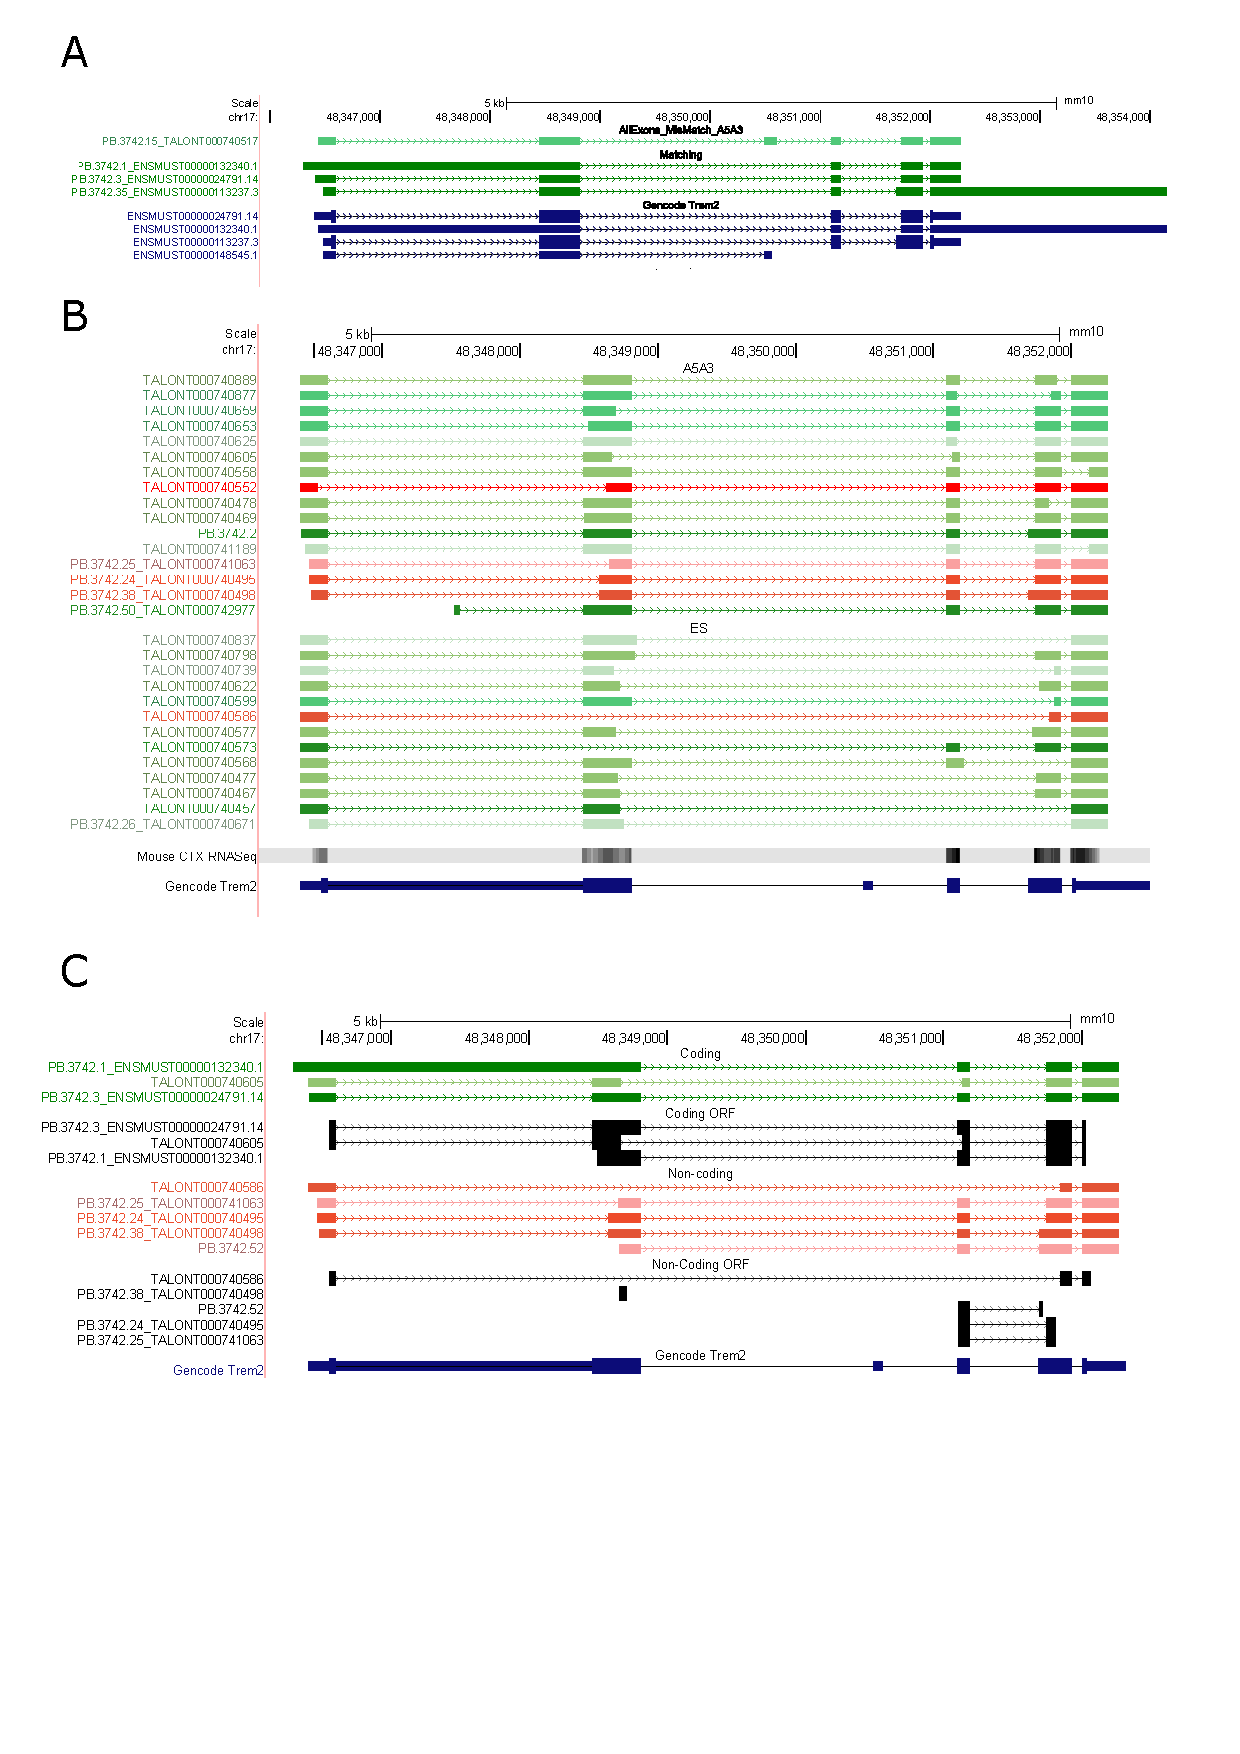
\includegraphics[page=1,trim={1cm 6cm 0 0},scale = 0.85]{Figures/pdfjoiner.pdf}
	\end{center}
	\captionsetup{width=0.95\textwidth}
	\caption[Trem2]%
	{\textbf{}: }   
	\label{fig:trem_track1}
\end{figure}

\begin{figure}[htp]
	\begin{center}
		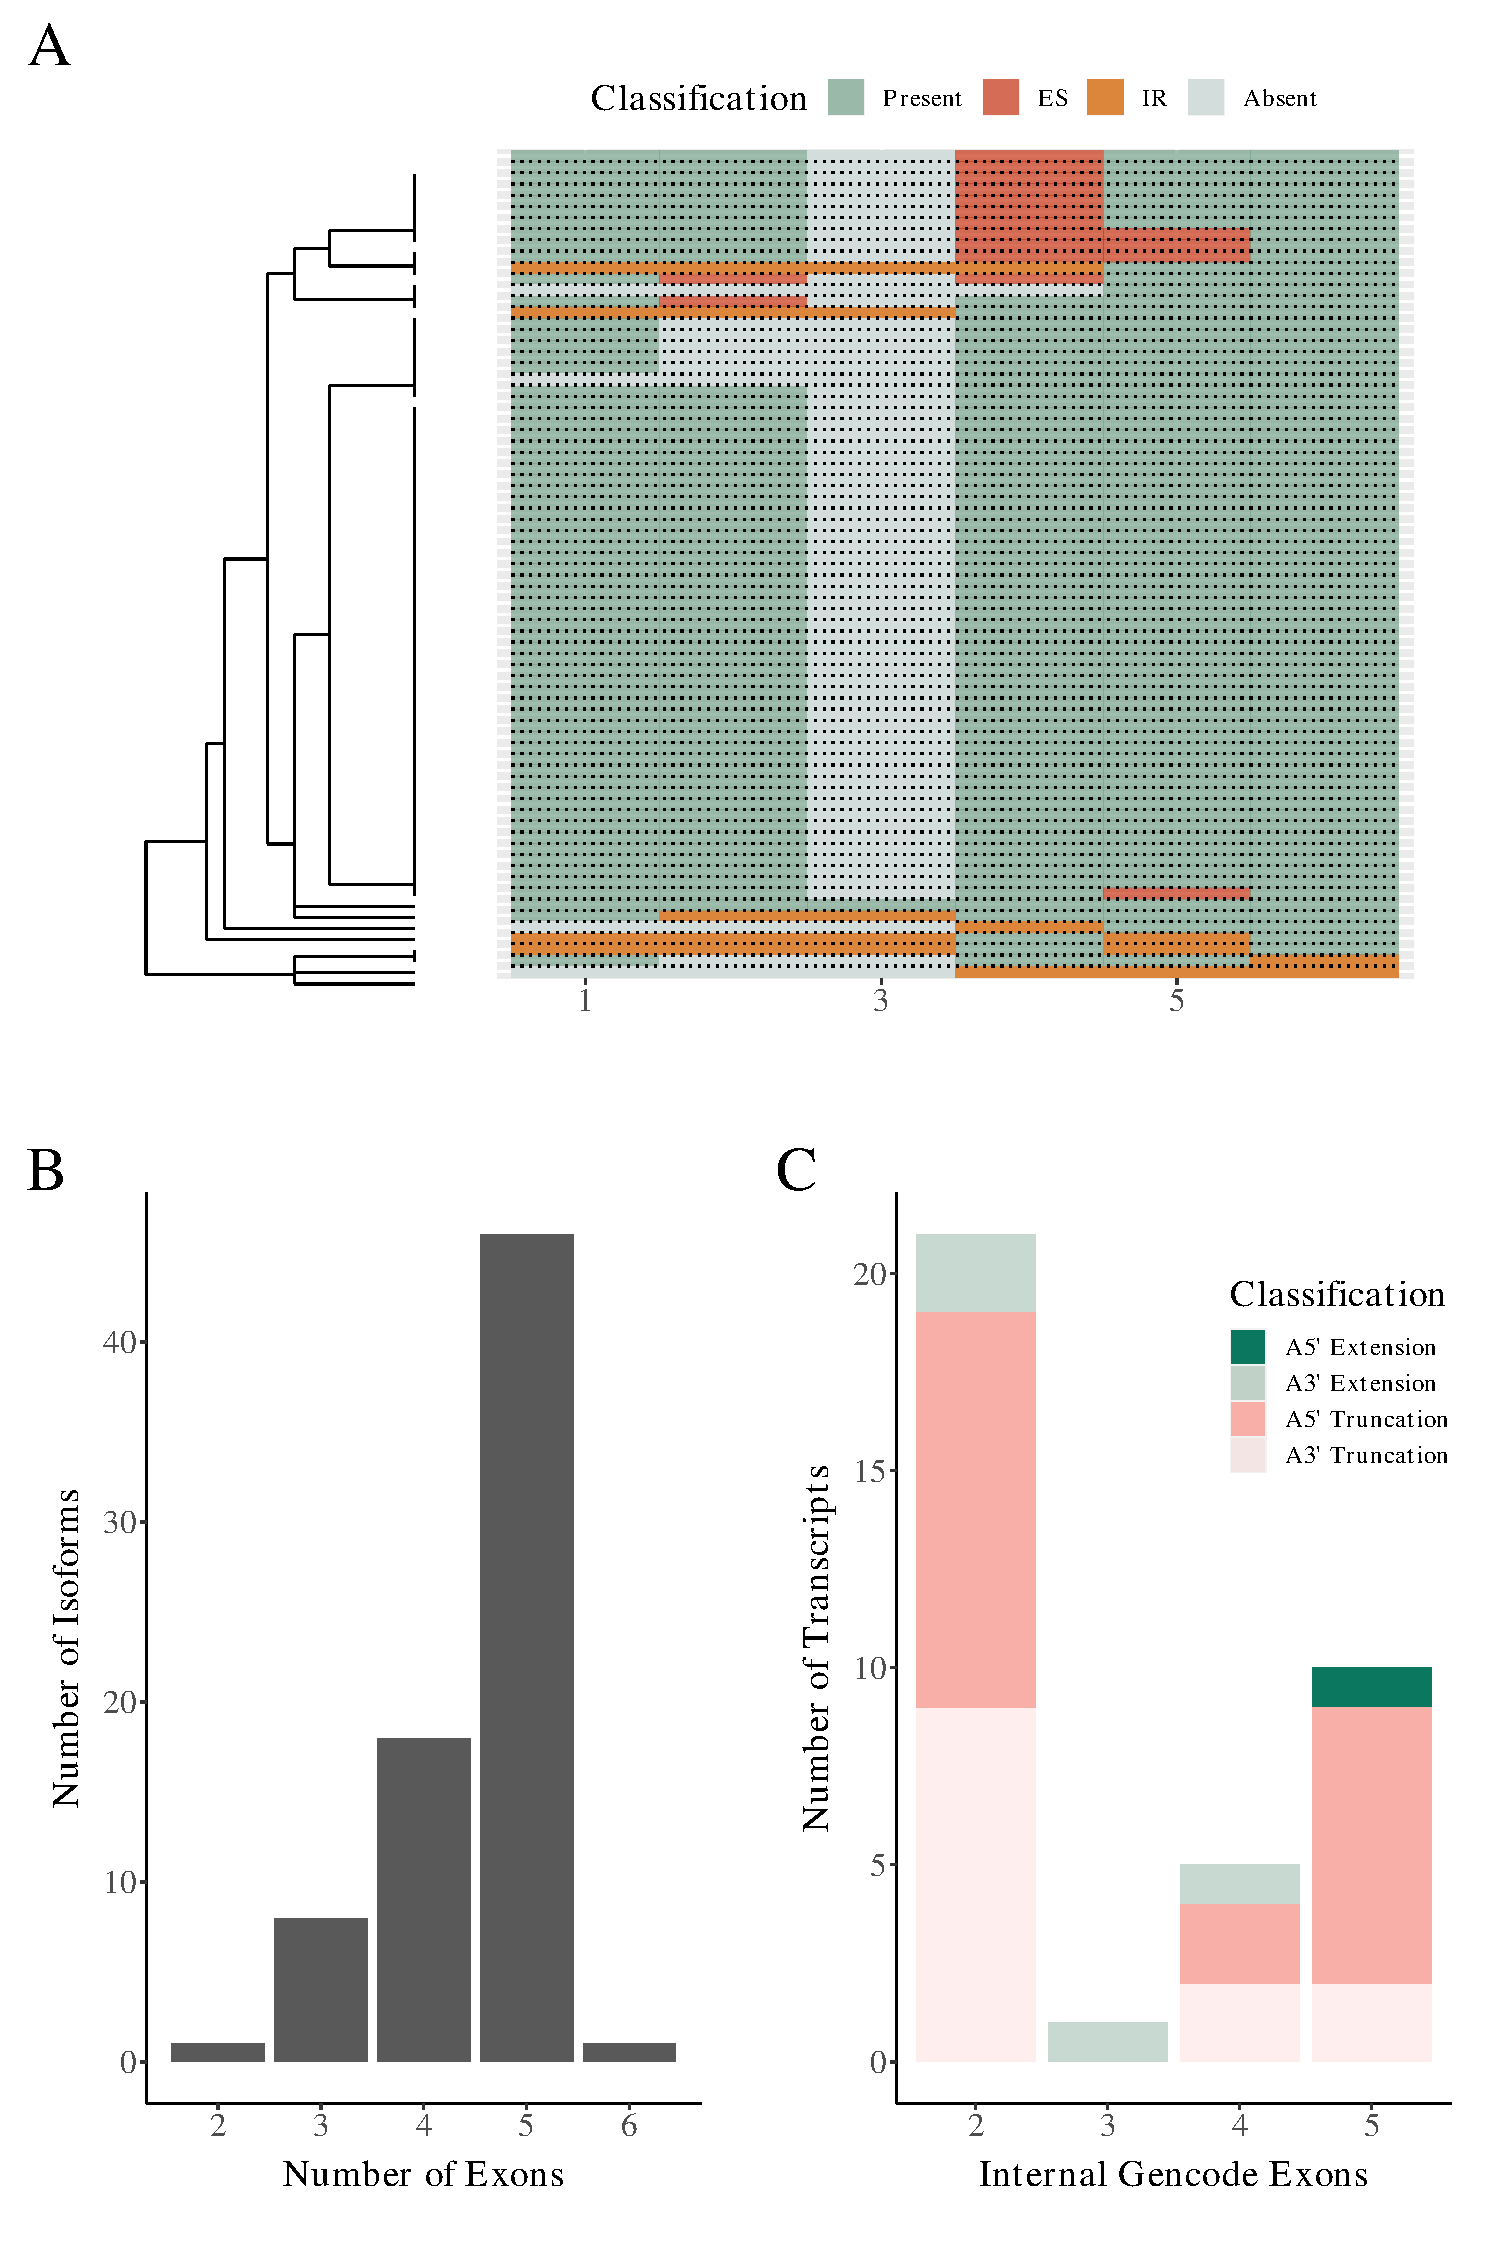
\includegraphics[page=1,trim={1cm 1cm 0 2cm},scale = 0.55]{Figures/TargetGenes.pdf}
	\end{center}
	\captionsetup{width=0.95\textwidth}
	\caption[Trem2]%
	{\textbf{}: }   
	\label{fig:trem}
\end{figure}

\begin{landscape}
	\begin{figure}[htp]
		\begin{center}
			\includegraphics[page=2,trim={0 4cm 0 0},scale = 0.85]{Figures/pdfjoiner.pdf}
		\end{center}
		\captionsetup{width=0.95\textwidth}
		\caption[RNA-Seq defined transcriptome]%
		{\textbf{}: }   
		\label{fig:trem_track2}
	\end{figure}
\end{landscape}

Using the merged full-length read count as a proxy for isoform abundance, one of the canonical isoform (XXX) was found to be most abundance with an abundance of XX-XX\% across all samples. Grouping the isoforms by splicing patterns, isoforms with all five exons accounted for XX\% of abundance. Corroborating previous findings that intron-retained transcripts with less abundantly expressed, isoforms with intron retention accounted for XX\% of abundance.

% Note: Crosstalk between Cd33 and Trem2 in 5xFAD
%% Differential expression in microglia, cross-reference results: https://actaneurocomms.biomedcentral.com/articles/10.1186/s40478-020-01099-x

\subsubsection{Abca7}
In total, we detected 41 isoforms associated with \textit{Abca7}. Reflecting the similarity of the 3 known isoforms, four novel isoforms were also identified with all the exons and only differed slightly with <10bp "wobble" within the internal structure (\cref{fig:abca7_track}). In contrast to these long isoforms, we detected significantly shorter isoforms that broadly fell into 2 categories: 1) isoforms that preserved the exonic structure at the 5'start with a truncated end accompanied by intron retention (n = 5 isoforms, 12.2\%), and 2) isoforms with preserved exonic structure at the 3'end and an enrichment of both exon skipping and intron retention (n = 23, 56\%) (\cref{fig:abca7_track}). While the isoforms with matching 3'end could be novel isoforms generated from an alternative promoter, they could also be artefacts generated from the 5' degradation. Nonetheless, we found exon skipping to be exclusive to either exon 31 (n = 1, XX\%) and exon 32 (n = XX\%) (\cref{fig:abca7}), both of which encode for the ATP binding cassette. Similarly, while intron retention was more widespread across the length of the gene, we observed intron retention particularly to be enriched between exon 37 and exon 39(\cref{fig:abca7}, \cref{fig:abca7_track}). 
%check AUG promoter 

\begin{landscape}
	\begin{figure}[htp]
		\begin{center}
			\includegraphics[page=3,trim={0 6cm 0 0},scale = 0.85]{Figures/pdfjoiner.pdf}
		\end{center}
		\captionsetup{width=0.95\textwidth}
		\caption[RNA-Seq defined transcriptome]%
		{\textbf{}: }   
		\label{fig:abca7_track}
	\end{figure}
\end{landscape}

\begin{figure}[htp]
	\begin{center}
		\includegraphics[page=2,trim={0 21cm 0 0cm},scale = 0.55]{Figures/TargetGenes.pdf}
	\end{center}
	\captionsetup{width=0.95\textwidth}
	\caption[Trem2]%
	{\textbf{}: }   
	\label{fig:abca7}
\end{figure}


\begin{landscape}
	\begin{figure}[htp]
		\begin{center}
			\includegraphics[page=4,trim={0 7cm 0 0},scale = 0.85]{Figures/pdfjoiner.pdf}
		\end{center}
		\captionsetup{width=0.95\textwidth}
		\caption[RNA-Seq defined transcriptome]%
		{\textbf{}: }   
		\label{fig:abca7_orf}
	\end{figure}
\end{landscape}


\subsubsection{Abca1}
Despite detecting far fewer isoforms associated with \textit{Abca1} (n = 7, \cref{fig:abca1}\textbf{A}) compared to \textit{Abca7} (n = 41), we also observed occurrence of exon skipping and intron retention events. Notably, we detected an isoform that spanned the length of the known canonical isoform (ENSMUST00000030010.3) using both PacBio Iso-Seq and ONT, but skipped two exons (exon 24 and exon 35) and harboured a novel exon next to one of the skipped exons (between exon 24 and exon 25, \cref{fig:abca1}\textbf{B,C}). Skipping of exon 35, which encodes for the ABC2 membrane 3 (\textit{Abca1} transmembrane domain), was also observed in one of the shorter isoforms. ORF prediction showed skipping of such exons shortened but maintained the open reading frame, and inclusion of the novel exon did not translate to additional protein domains. Lastly, we identified two shorter isoforms with premature termination accompanied with intron retention (\cref{fig:abca1}\textbf{A,B}). ORF prediction of such transcripts similarly showed a shortened but maintained open reading frame with no prediction of NMD. 

\subsubsection{Trpa1}
From the panel of AD-associated genes enriched in the rTg4510 mouse cortex, \textit{Trpa1} - the ion channel receptor - was the least abundant and characterised with the fewest number of isoforms (n = 4) (\cref{fig:rhbdf2}\textbf{A}). Aside from detecting one of the two known canonical isoforms (Trpa1-201, ENSMUST00000041447.4), we further identified 2 novel isoforms that spanned the full-length of the known isoform and a short non-coding novel isoform (\cref{fig:rhbdf2}\textbf{A,B}). Blast analysis of the 2 novel isoforms and known isoform revealed that the exonic structure was generally conserved across the gene, with the exception of skipping of exon 20, varying lengths of the 5' and 3' UTR, and a 4-nucleotide addition at the end of exon 6 (\cref{fig:rhbdf2}\textbf{C}); RNA-Seq data from matched samples validate this 3' extension. 

ORF prediction of skipping of exon 20, which encodes for part of the ion channel domain, shortened but maintained the reading frame. However, strikingly, the most well-predicted ORF of the two novel isoforms was shifted significantly with initiation at a downstream AUG codon (\cref{fig:rhbdf2}\textbf{A}). Further examination of the ORF predicted using \textit{CPAT} revealed two alternative ORF initiated from the upstream AUG codon, but resulted in premature termination with an in-frame stop codon due to the addition of 4 nucleotides at exon 6. Conversely, the reading frame was intact for the known isoform.             

\subsubsection{Rhbdf2}
The second least expressed gene within the panel of AD-associated target genes, \textit{Rhbdf2} was characterised with 5 isoforms and the least complex splicing pattern. Identifying two novel isoforms that spanned the length of the known detected canonical isoform (\cref{fig:rhbdf2}\textbf{A}), we detected exon skipping of exon 3 and exon 18 (\cref{fig:rhbdf2}\textbf{B}). While ORF prediction showed that all the isoforms generated a significantly shorter reading frame with usage of a downstream start codon, skipping of exon 18 resulted in a shorter terminal exon, which encoded for the rhomboid domain and is conserved in human (\cref{fig:rhbdf2}\textbf{A}). Similarly, the novel transcript with skipping of exon 3 had a shifted reading frame, however it was difficult to determine whether this was due to exon skipping or presence of an alternative first exon. Lastly, we detected a novel isoform that contained all the exons and was almost identical to the known isoform bar the deletion of 5 nucleotides from exon 7, which encodes for the protease domain. Strikingly, ORF prediction of this transcript revealed that this 3' truncation was accompanied with an even shorter reading frame (\cref{fig:rhbdf2}\textbf{C}).   

\subsubsection{Ank1} 
From the panel of AD-associated target genes, \textit{Ank1} stood out for the domination of significantly shorter known canonical isoforms (\cref{fig:Ank1_track}\textbf{A}). While we did detect several longer known canonical isoforms (n = 4, 23.5\%, length = 6.5 - 8.2kb), the majority (n = 11, 64.7\%) were less than \textasciitilde 2kb long and spanned the last few exons. Furthermore, the two most-abundant isoforms annotated to \textit{Ank1} using both PacBio Iso-Seq and ONT were one of the short known isoforms (Ank1-208, ENSMUST00000121075.7) and the short non-coding isoform (Ank1-211, ENSMUST00000130311.1). %Although we are unable to rule out the technical limits of sequencing the longer transcripts, given that \textit{Ank1} is one of the longer genes from the panel of target genes,  

Aside from the length disparities among the isoforms detected, we found that the splicing pattern was generally conserved across the gene with consistent skipping of certain exons (\cref{fig:Ank1}\textbf{B}). Across all the long isoforms, exon 44 was skipped whereas exon 46 was skipped in half of the short isoforms (n = 4). While ORF prediction showed that skipping of the earlier exons shortened but maintained the reading frame, inclusion of exon 44 resulted in the inclusion of a stop codon and resulted in premature termination with predicted NMD. Conversely, isoforms that skipped exon 44 maintained the reading frame to the final exon and was not predicted for NMD  
(\cref{fig:Ank1_track}\textbf{B}).        

\begin{landscape}
	\begin{figure}[htp]
		\begin{center}
			\includegraphics[page=5,trim={0 4cm 0 0},scale = 0.85]{Figures/pdfjoiner.pdf}
		\end{center}
		\captionsetup{width=1.5\textwidth}
		\caption[Visualisation of \textit{Abca1} isoforms]%
		{\textbf{Visualisation of \textit{Abca1} isoforms}: \textbf{A)} Shown is the UCSC genome browser track of \textit{Abca1}. Occurrence of exon skipping (ES) is boxed in purple. Isoforms are coloured based on coding status and shaded by abundance. Reference transcripts (blue), RNA-Seq data from matched samples, and Pfam domains are also shown. \textbf{B)} cluster dendrogram and visualisation of exon distribution, and \textbf{C)} an zoomed in figure of the browser track to illustrate skipping of exon 24 (boxed in purple) and inclusion of a novel exon (outlined in blue).}   
		\label{fig:abca1}
	\end{figure}
\end{landscape}

\begin{landscape}
	\begin{figure}[htp]
		\begin{center}
			\includegraphics[page=6,trim={0 5cm 0 0},scale = 0.85]{Figures/pdfjoiner.pdf}
		\end{center}
		\captionsetup{width=1.5\textwidth}
		\caption[Visualisation of \textit{Trpa1} isoforms]%
		{\textbf{Visualisation of \textit{Trpa1} isoforms}: \textbf{A)} Shown is the UCSC genome browser track of \textit{Trpa1}. Occurrence of exon skipping (ES) is boxed in purple. Isoforms are coloured based on coding status and shaded by abundance. Reference transcripts (blue), RNA-Seq data from matched samples, and Pfam domains are also shown. \textbf{B)} cluster dendrogram and visualisation of exon distribution of 4 isoforms annotated to \textit{Trpa1}. \textbf{C)} Zoomed in figure of the browser track to illustrate the addition of 4 nucleotides (GCAA, highlighted in pink) to exon 6 of the 2 novel isoforms, resulting in a truncated ORF destined for NMD (denoted with pink circle). NMD - nonsense mediated decay, ORF - Open reading frame.}   
		\label{fig:trpa1}
	\end{figure}
\end{landscape}

\begin{landscape}
	\begin{figure}[htp]
		\begin{center}
			\includegraphics[page=7,trim={0 5cm 0 0},scale = 0.85]{Figures/pdfjoiner.pdf}
		\end{center}
		\captionsetup{width=1.5\textwidth}
		\caption[Visualisation of \textit{Rhbdf2} isoforms]%
		{\textbf{Visualisation of \textit{Rhbdf2} isoforms}: \textbf{A)} Shown is the UCSC genome browser track of \textit{Rhbdf2}. Occurrence of exon skipping (ES) is boxed in purple. Isoforms are coloured based on coding status and shaded by abundance. Reference transcripts (blue), RNA-Seq data from matched samples, Pfam domains, and the most well-predicted ORF (black) are also shown. \textbf{B)} cluster dendrogram and visualisation of exon distribution of 5 isoforms annotated to \textit{Rhbdf2}. \textbf{C)} Zoomed in figure of the browser track to illustrate the deletion of 5 nucleotides (GTAAG, highlighted in pink) to exon 7 of the 2 novel isoforms, resulting in a truncated ORF. NMD - nonsense mediated decay, ORF - Open reading frame.}   
		\label{fig:rhbdf2}
	\end{figure}
\end{landscape}

\begin{landscape}
	\begin{figure}[htp]
		\begin{center}
			\includegraphics[page=8,trim={0 2cm 0 0},scale = 0.85]{Figures/pdfjoiner.pdf}
		\end{center}
		\captionsetup{width=1.5\textwidth}
		\caption[Visualisation of \textit{Ank1} isoforms]%
		{\textbf{Visualisation of \textit{Ank1} isoforms}: }   
		\label{fig:Ank1_track}
	\end{figure}
\end{landscape}
\begin{figure}[t]
	\captionsetup{width=0.95\textwidth}
	\contcaption{\textbf{Visualisation of \textit{Ank1} isoforms}: \textbf{A)} Shown is the UCSC genome browser track of \textit{Ank1}. Isoforms are coloured based on coding status and shaded by abundance. Reference transcripts (blue), RNA-Seq data from matched samples, Pfam domains, and the most well-predicted ORF (black) further classified by NMD prediction are also shown. \textit{B)} Zoomed in figure of the browser track to illustrate the skipping of exon 46 and subsequent shifting of reading frame to avoid NMD. NMD - nonsense mediated decay, ORF - Open reading frame.}%
\end{figure}

\begin{figure}[htp]
	\begin{center}
		\includegraphics[page=6,trim={1cm 1cm 0 2cm},scale = 0.55]{Figures/TargetGenes.pdf}
	\end{center}
	\captionsetup{width=0.95\textwidth}
	\caption[Characterisation of \textit{Ank1} with multiple exon skipping events]%
	{\textbf{Characterisation of \textit{Ank1} with multiple exon skipping events}: \textbf{A)} Cluster dendrogram and visualisation of exon distribution of 17 isoforms annotated to \textit{Ank1}, characterised with exon skipping of multiple exons. \textbf{B)} Number of isoforms for each exon skipped}   
	\label{fig:Ank1}
\end{figure}

\newpage
\subsubsection{Cd33}
In total, we detected 41 isoforms associated with \textit{Cd33}, including 5 of the known isoforms (\cref{fig:cd33_track}). Reflecting the diversity of \textit{Cd33} known isoforms, the majority of isoforms detected were similarly short, lacked the first two upstream exons and also skipped exon 8 which was only present in the Cd33-201 known isoform (ENSMUST00000004728.11) (\cref{fig:Cd33}\textbf{A}, \cref{fig:cd33_track}). ORF predictions showed that skipping of this exon slightly reduced but maintained the reading frame (\cref{fig:cd33_track2}\textbf{A}). Conversely, 3'truncation of exon 4 (which encodes for the V-set domain) shifted the reading frame with the generation of a stop codon and subsequent usage of the downstream initiator codon in exon 2 (\cref{fig:cd33_track2}\textbf{A}).   

While the majority of isoforms were short, we detected a few novel, "full-length" isoforms that incorporated different features from the reference isoform (\cref{fig:cd33_track2}\textbf{B}); i.e. contained the upstream exons only present in the Cd33-202 known isoform (ENSMUST00000039861.6) while harbouring the longer 3'UTR present in the Cd33-203 known isoform (ENSMUST00000205503.1). Notably, we detected two very similar "full-length" isoforms that both contained a novel upstream exon between exons 1 and 2 (66bp, Chr7:43529866-43529932, \cref{fig:cd33_track2}\textbf{B}). However strikingly, due to similar 3' truncation of exon 4, ORF prediction of these two isoforms similarly revealed a shortened reading frame starting from exon 2 despite the presence of upstream exons.  

In contrast to exon skipping, we observed multiple intron retention events (IR) across the gene with over a third of isoforms (n = 14, 34.21\%) containing at least one IR event (\cref{fig:Cd33}\textbf{B}), and one isoform containing an intron retention event that spanned 4 exons (TALONT001237573, \cref{fig:cd33_track2}\textbf{C}). Further examination revealed that intron retention primarily occurred around exon 7 (\cref{fig:Cd33}\textbf{A}) and extended to the final two exons, exon 8 and 9, with varying lengths (\cref{fig:cd33_track2}\textbf{C}). ORF predictions showed that an extended intron retention at exon 7 revealed a stop codon resulting in a shortened reading frame, whereas an intact exon 7 resulted in a slightly longer reading frame.

\begin{figure}[htp]
	\begin{center}
		\includegraphics[page=7,trim={1cm 0cm 0 2cm},scale = 0.55]{Figures/TargetGenes.pdf}
	\end{center}
	\captionsetup{width=0.95\textwidth}
	\caption[Characterisation of \textit{Cd33} with multiple intron retained events]%
	{\textbf{Characterisation of \textit{Cd33} with multiple intron retained events}: \textbf{A)} Cluster dendrogram and visualisation of exon distribution of 41 isoforms annotated to \textit{Cd33}, characterised with intron retention of multiple exons. \textbf{B)} Number and percentage of isoforms that spanned the number of exons with intron retention. \textbf{C)} Number and percentage of isoforms with intron retention of the exon. "IR" refers to the sole intron retention of that exon, whereas "IRMatch" refers to presence of an intron retention event that spanned over more than one exon. 
	}   
	\label{fig:Cd33}
\end{figure}

\begin{landscape}
	\begin{figure}[htp]
		\begin{center}
			\includegraphics[page=9,trim={0 13cm 0 0},scale = 0.85]{Figures/pdfjoiner.pdf}
		\end{center}
		\captionsetup{width=1.5\textwidth}
		\caption[Visualisation of \textit{Cd33} isoforms]%
		{\textbf{Visualisation of \textit{Cd33} isoforms}: \textbf{A)} Shown is the UCSC genome browser track of \textit{Cd33}. Isoforms are coloured based on coding status and shaded by abundance. Reference transcripts (blue), RNA-Seq data from matched samples, Pfam domains, and the most well-predicted ORF (black) are also shown}   
		\label{fig:cd33_track}
	\end{figure}
\end{landscape}

\begin{landscape}
	\begin{figure}[htp]
		\begin{center}
			\includegraphics[page=10,trim={0 4cm 0 0},scale = 0.85]{Figures/pdfjoiner.pdf}
		\end{center}
		\captionsetup{width=1.5\textwidth}
		\caption[Visualisation of \textit{Cd33} isoforms]%
		{\textbf{Visualisation of \textit{Cd33} isoforms}: \textbf{A)} Shown is the UCSC genome browser track of \textit{Cd33} with skipping of exon 8 (shaded in purple). Truncation of exon 4 (shaded in red) resulting in shifted reading frame and subsequent usage of downstream initiator codon is depicted with red arrow. \textbf{B)} Detection of "full-length" isoforms with detection of two novel exons (shaded in blue). \textbf{C)} Detection of multiple intron retention events with enriched occurrence at exon 7. The isoform (TALONT001237573) with intron retention spanning across 4 exons is denoted by asterisk and shaded in yellow.}   
		\label{fig:cd33_track2}
	\end{figure}
\end{landscape}

\subsubsection{Sorl1}
Although we detected 113 isoforms associated with \textit{Sorl1} - a gene which encodes for the endocytic receptor involved in APP trafficking - the splicing pattern was relatively simple with the internal exonic structure largely conserved and only a few isoforms exhibiting exon skipping and intron retention events (\cref{fig:sorl1}\textbf{A}, \cref{fig:sorl1_track1}). Strikingly, isoform diversity was primarily driven by usage of alternative promoter and termination usage while preserving the internal exonic structure (\cref{fig:sorl1_track2}\textbf{A}). Over 75\% (n = 88, 77.9\%) of the isoforms detected were characterised with a slightly different downstream first exon, which can be further broadly classified into three groups by presence of an alternative last exon at exons 37, 38 and 41 (\cref{fig:sorl1_track2}\textbf{B}). Furthermore, the alternative last exons do not fully match the exon of interest, resulting in enrichment of isoforms with A3' truncation of exon 37, 38, and 41 (\cref{fig:sorl1}\textbf{B}). Notably, exons 37 and 38 encode for Fibronectin type III domain, which is the largest protein domain of the SORL1 protein, and of which studies have previously identified rare AD-associated variants to be located within\cite{Verheijen2016}. ORF prediction of these isoforms with alternative promoter and terminator usage show shortened but otherwise intact reading frames with no prediction for NMD. 

\begin{figure}[htp]
	\begin{center}
		\includegraphics[page=8,trim={1cm 0cm 0 2cm},scale = 0.55]{Figures/TargetGenes.pdf}
	\end{center}
	\captionsetup{width=0.95\textwidth}
	\caption[Characterisation of \textit{Sorl1} with extensive alternative promoter usage]%
	{\textbf{Characterisation of \textit{Sorl1} with extensive alternative promoter usage}: \textbf{A)} Cluster dendrogram and visualisation of exon distribution of 113 isoforms annotated to \textit{Sorl1}, characterised with extensive alternative promoter usage. \textbf{B)} Number of isoforms with A5' and A3' truncation and extension.
	}   
	\label{fig:sorl1}
\end{figure}

\begin{landscape}
	\begin{figure}[htp]
		\begin{center}
			\includegraphics[page=11,trim={0 11cm 0 0},scale = 0.85]{Figures/pdfjoiner.pdf}
		\end{center}
		\captionsetup{width=1.5\textwidth}
		\caption[Visualisation of \textit{Sorl1} isoforms]%
		{\textbf{Visualisation of \textit{Sorl1} isoforms}: \textbf{A)} Shown is the UCSC genome browser track of \textit{Sorl1} with exon skipping (shaded in purple) and intron retention (shaded in yellow). Isoforms are coloured based on coding status and shaded by abundance. Reference transcripts (blue), RNA-Seq data from matched samples, Pfam domains, and the most well-predicted ORF (black) are also shown.}   
		\label{fig:sorl1_track1}
	\end{figure}
\end{landscape}

\begin{figure}[htp]
	\begin{center}
		\includegraphics[page=12,trim={0 6cm 0 0},scale = 0.85]{Figures/pdfjoiner.pdf}
	\end{center}
	\captionsetup{width=0.95\textwidth}
	\caption[Visualisation of \textit{Sorl1} isoforms]%
	{\textbf{Visualisation of \textit{Sorl1} isoforms}: \textbf{A)} Shown is the UCSC genome browser track of \textit{Sorl1} with extensive alternative promoter and terminator usage. \textbf{B)} While the isoforms greatly differ at the 5' end, the 3' ends of such isoforms are conserved with alternative termination at exons 37, 38 (outlined in blue) and 41 (outlined in pink).}   
	\label{fig:sorl1_track2}
\end{figure}

\newpage
\subsubsection{Vgf}
We detected 90 isoforms associated with \textit{Vgf}, despite it only containing 5 exons. Examination of this gene, which encodes for a neurosecretory protein that is cleaved into various peptides, remarkably suggested a relatively simple splicing pattern (\cref{fig:vgf}\textbf{A}): no detection of the first two upstream exons present in only one of the known isoform, the majority of isoforms skipped exon 5 and a few intron retention events were observed. However, further examination revealed complex variations of the final exon and 3'UTR (\cref{fig:vgf}\textbf{B})), as supported by matched RNA-Seq data (\cref{fig:vgf_track}). The vast majority of isoforms detected (n = 87, 96.7\%) were characterised with either an alternative 5' start sites (n = 35 isoforms, 38.9\%) or 3'end of the last exon (n = 4, 0.04\%), or with matched 5' and 3' end sites but skipping within the exon resulting in two enclosed exons (\cref{fig:vgf_track}). This phenomenon of skipping within the exon further extended beyond exon 6 in a few intron-retained isoforms. Given that isoforms exhibiting this "internal exon skipping" were detected in both PacBio Iso-Seq and ONT with stringent filtering, these are unlikely to be artefacts. 

ORF predictions of these isoforms showed that while this internal skipping phenomenon did not result in NMD, it generated significant variations of the reading frame particularly at the 3'end. Conversely, isoforms with alternative 5' start site of the last exon were predicted as either non-coding or missing an ORF.

\begin{figure}[htp]
	\begin{center}
		\includegraphics[page=10,trim={1cm 1cm 0 2cm},scale = 0.55]{Figures/TargetGenes.pdf}
	\end{center}
	\captionsetup{width=0.95\textwidth}
	\caption[Characterisation of \textit{Vgf} with extensive alternative last exon]%
	{\textbf{Characterisation of \textit{Vgf} with extensive alternative last exon}: \textbf{A)} Cluster dendrogram and visualisation of exon distribution of 90 isoforms annotated to \textit{Vgf} \textbf{B)} Number of isoforms with A5' and A3' truncation and extension.
	}   
	\label{fig:vgf}
\end{figure}


\begin{figure}[htp]
	\begin{center}
		\includegraphics[page=13,trim={0 12cm 0 0},scale = 0.85]{Figures/pdfjoiner.pdf}
	\end{center}
	\captionsetup{width=0.95\textwidth}
	\caption[Visualisation of \textit{Vgf} isoforms]%
	{\textbf{Visualisation of \textit{Vgf} isoforms:} Shown is the UCSC genome browser track of \textit{Vgf} with extensive variation of the last exon.}   
	\label{fig:vgf_track}
\end{figure}

\newpage
\subsubsection{Fyn}
Known to directly phosphorylate and interact with tau, \textit{Fyn} encodes for a tyrosine kinase that is associated with several known isoforms that primarily differ in the first exon from usage of alternative promoter. Detecting in total 50 isoforms, we found these first exons to be mutually exclusive with either isoforms containing exon 1, 2 or 4 (\cref{fig:fyn}). In contrast, we did not detect the shorter isoforms with the most downstream alternative promoter at exon 5 or 6. However, we did detect a significant number of isoforms (n = XX) that contained novel first exons at 3 distinct positions; between exons 2 and 3, 4 and 5, and even further downstream at exon 8. Strikingly, the novel exon between exons 4 and 5 was found in isoforms with alternative 4 exon, highlighting the complexity of alternative promoter usage in \textit{Fyn}. Of note, ORF predictions of these isoforms with novel exons did not change the reading frame, and similarly exon skipping shortened but otherwise maintained reading frame.  

In contrast to the complexity at the 5'end of the gene, the exonic structure downstream of exon 7 was relatively conserved across the majority of isoforms. Particularly exons between exon 7 and 12, which encode for the SH3 domain known to interact with tau, were present across all the isoforms (\cref{fig:fyn_track}). Conversely, exons 13 and 14,  which encode for the protein kinase domain, were found to be mutually exclusive with the majority of detected isoforms containing exon 13 (n = 36) and skipping exon 14 (\cref{fig:fyn_track}). Finally, we noted a complete absence of exon 16, which originated from an alternative first exon of the shortest known isoform. 

\begin{figure}[htp]
	\begin{center}
		\includegraphics[page=9,trim={1cm 20cm 0 2cm},scale = 0.55]{Figures/TargetGenes.pdf}
	\end{center}
	\captionsetup{width=0.95\textwidth}
	\caption[Characterisation of \textit{Fyn} with alternative first exon and alternative promoter usage]%
	{\textbf{Characterisation of \textit{Fyn} with alternative first exon and alternative:} Cluster dendrogram and visualisation of exon distribution of 50 isoforms annotated to \textit{Fyn}
	}   
	\label{fig:fyn}
\end{figure}

\begin{landscape}
	\begin{figure}[htp]
		\begin{center}
			\includegraphics[page=14,trim={0 5cm 0 0},scale = 0.85]{Figures/pdfjoiner.pdf}
		\end{center}
		\captionsetup{width=1.5\textwidth}
		\caption[Visualisation of \textit{Fyn} isoforms]%
		{\textbf{Visualisation of \textit{Fyn} isoforms:} Shown is the UCSC genome browser track of \textit{Fyn}}   
		\label{fig:fyn_track}
	\end{figure}
\end{landscape}


\subsubsection{Picalm}
In total, we detected 144 isoforms associated with \textit{Picalm}, a gene that encodes for an adaptor protein that is involved with APP trafficking and endocytosis. Of these 144 isoforms, we identified all the known isoforms, including the mono-exonic isoforms, bar the non-coding isoform Picalm-208	 (ENSMUST00000207949.1). Approximately a fifth of the isoforms (n = 31, 21.5\%) detected spanned the "full-length" of the gene from exon 1 to 21, while the remaining isoforms were significantly shorter with alternative first exon and promoter usage from every exon. Of note, we identified a novel isoform that contained a novel first exon 59kb upstream of known exon 1 and was detected using both PacBio Iso-Seq and ONT (PB.7635.2-TALONT001254093).
	
While exon skipping was observed consistently at exons 13, 18, and 21, which do not encode for any Pfam domains, the internal exonic structure was broadly conserved. ORF predictions showed that skipping of such exons shortened but maintained the reading frame. \textit{Picalm} isoform diversity was subsequently driven by usage of alternative first exon and promoter. Such shorter isoforms are unlikely to be artefacts given that a few of the known isoforms display similar feature (i.e partial subset of the longer "full-length" isoforms), a significant number (n = 66, 60\%) were detected using both long-read sequencing approaches, and after performing stringent filtering. 
	
%However, the vast majority of coding isoforms were predicted to undergo nonsense mediated decay (n = 115, 98.3\%) including the known reference isoforms. Further examination revealed that while the reading frame varied at the 5'end from alternative first exon usage, all the reading frames 

\begin{figure}[htp]
	\begin{center}
		\includegraphics[page=11,trim={1cm 20cm 0 2cm},scale = 0.55]{Figures/TargetGenes.pdf}
	\end{center}
	\captionsetup{width=0.95\textwidth}
	\caption[Characterisation of \textit{Picalm} with alternative first exon and alternative promoter usage]%
	{\textbf{Characterisation of \textit{Picalm} with alternative first exon and alternative promoter usage }: Cluster dendrogram and visualisation of exon distribution of 144 isoforms annotated to \textit{Picalm}.
	}   
	\label{fig:picalm}
\end{figure}

\subsubsection{Tardbp}
\textit{Tardbp} encodes for TDP-43, aggregates of which are frequently observed in multiple neurodegenerative diseases including ALS and FTD. Although not the primary hallmark of AD, up to 75\% of AD patients are also presented with TDP-43 aggregates. Despite only containing 10 exons, \textit{Tardbp} is one of the most complex gene from the targeted panel of AD-associated genes; various isoforms contain exon overlap at multiple regions at the 3'end from exon 6 onwards. The complexity is reflective of the "internal exon skipping" phenomenon observed in the final exon of \textit{Vgf}, with added complexity from additional usage of alternative termination and 3'sites of the last exon. This complexity was also captured in our targeted dataset with detection of known isoforms either with matching or slight wobble splice sites. We also detected novel isoforms with a combination of exons from different known isoforms; e.g. a novel isoform (PB.6120.170) that contained all the exons from ENSMUST00000190287.1 and the upstream first three exons from the longer "full-length" known isoforms. 

Despite the complexity of the 3'end of \textit{Tardbp}, we observed a relatively consistent splicing pattern with multiple intron retention events, particularly between exons 6 and 7. A XX of isoforms were also identified with an alternative last exon accompanied with terminal intron retention at exons 7 and 8. Conversely, exons 2 to 4, which encode for RNA recognition motif domain were present and structurally preserved in the majority of isoforms.  



\subsubsection{Mapt}
The aggregation of tau, which is encoded by \textit{Mapt}, into neurofibrillary tangles is one of the two key hallmarks of AD. To study splicing changes associated with progression of tau pathology, we used rTg4510 mouse model which harbours the human tau transgene, Mapt\textsuperscript{P301L}. As previously shown, human-specific \textit{MAPT} transcripts were only detected in TG mice and were removed for downstream analysis, retaining only mouse-specific \textit{Mapt} transcripts. 

In total, we detected 140 isoforms associated with \textit{Mapt}, including 7 of the known isoforms. Upon further examination of these isoforms, one of the most striking splicing feature observed was the number of consistent exon skipping events that alternated across the gene. The majority of isoforms were characterised with at least one exon skipping event (n = 115, 82.1\%) with most isoforms skipping 3 exons or more (n = 98); notably, we detected an isoform with extensive skipping of 12 exons. Despite the widespread occurrence of exon skipping, we found that the splicing pattern was conserved across the isoforms with skipping of alternative exons; i.e. exons 4, 6, 8, 10 and 13. In contrast, exons 2, 7, 11, 12 and 14, which were present in all the known isoforms (i.e. constitutive) were also present in all the isoforms that spanned the "full-length" of the gene. 

Detected in both PacBio Iso-Seq and ONT, we identified a number of isoforms with novel first exons located between exon 1 and 2 (n = 16, 11.4\%), which were broadly clustered into five groups and indicated alternative promoter usage. Notably, some of these novel exons were also contained within the other isoforms. ORF prediction of these isoforms showed that usage of these alternative first exons shortened but maintained the reading frame. 

Finally, we detected some significantly shorter isoforms that were distinguished by the presence of a intron-retained first exon. These broadly appeared between exons 9 and 11 which encode for the tubulin-binding repeat domain. 

\subsubsection{Fus}
Identified as a causative gene for amyotrophic lateral sclerosis (ALS) and FTD, \textit{Fus} has become the characteristic pathological hallmark for neuronal aggregation in the subset of sporadic FTD cases that lack the more established inclusion markers of TDP-43 and tau\cite{Seelaar2010}. Despite only containing 15 exons, \textit{Fus} is a complex gene; multiple isoforms with varying lengths and exon inclusion are generated with only a quarter of the known isoforms (n = 4, 25\%) spanning the full-length of the gene. In total, we detected a total of 236 isoforms annotated to \textit{Fus}, the majority of which were "full-length" (n = 154, 58.6\%). Consequently in contrast to the known \textit{Fus} isoform landscape in the mouse genome, we found the \textit{Fus} splicing pattern relatively simpler in our dataset. A quarter (n = 53, 25.7\%) of the isoforms detected were largely analogous to the "full-length" isoform in preserving the exonic structure, differing by minor variations ("wobble") at the splice site. 

Nonetheless, we detected widespread occurrence of exon skipping and intron retention events that were not observed in the reference genome. Over 40\% of isoforms (n = 103, 43.6\%) were characterised with at least one exon skipping event, with exon 8 exclusion observed in almost half of the these isoforms (n = 50 isoforms with exon 8 skipped, n = 48.5\%). Around the same region, we also detected a number of isoforms with intron retention events spanning across exons 6 and 7, which are also identified in the novel isoforms. However notably, we noted an intron-retained isoform than incorporated one of the known mono-exonic isoforms, resulting in an intron retained region spanning exons 10-12 which encode the RNA recognition motif (RRM) domain. Finally, we detected a number of intron retention events at the 3'end of the gene between exons 12 and 14, which encode zinc-finger-containing RGG-Znf-RGG domain (zF-RanBP). As an RNA-binding protein and a subunit of the heterogeneous nuclear ribonucleoprotein complex (hnRNP) complex involved in splicing, FUS recognition of RNA is mediated by both the RRM and zF-RanBP domains\cite{Wang2015c}. 

\subsubsection{Bin1}
\textit{Bin1} has been well implicated in AD pathology through identification of multiple AD-associated SNPs from GWAS studies, and recent studies on human post-mortem AD brains have shed light on the function and differential expression of its associated isoforms\cite{Taga2020}. Drawing parallels to the human-equivalent \textit{Bin1} isoforms, we observed extensive exon skipping within certain parts of the gene; the majority of isoforms (n = 290 isoforms, 78.8\%) were characterised with at least one exon skipping event. The first 10 exons encoding the N-BAR domain, which is involved in membrane curvature, were conserved and included in the "full-length" isoforms. Conversely inclusion of exons 14-16, which encode the CLAP domain involved in endocytosis, was highly variable among isoforms (Exon 14 skipping: XX isoforms, Exon 15 skipping: XX isoforms, Exon 16 skipping: XX isoforms). However, intron retention events (n = XX) were also notably enriched within this region. Aside from detecting long isoforms spanning the full-length of the gene, we also detected shorter isoforms with exclusion of the initial exons encoding the N-BAR domain but inclusion of the terminal exons encoding the Src homology 3 (SH3) domains. Among these, a number of isoforms (n = 19, ) were relatively similar in length and exonic structure to Bin1-204 (ENSMUST00000234373.1) with a long alternative first exon encoding the CLAP domain.  

\subsubsection{App}
\textit{App}, encoding for amyloid precursor protein, is one of the most commonly involved gene for AD with \textasciitilde30 causative mutations described. Detecting a total of 466 isoforms annotated to \textit{App}, we observed varying isoform lengths with less than half of the isoforms (n = 183, 39.9\%) containing exon 1 and spanning the full length of the gene. While a number of isoforms were structurally analogous to the two known shorter isoforms - App-205 (ENSMUST00000227654.1) and App-210 (ENSMUST00000228375.1) - we detected a significant number that started with a novel alternative first exon between exons 3 and 5, which encode the APP heparin binding domain. Nonetheless, the variation typically resided within the 5' end of the gene with the vast majority of isoforms (n = 428, 91.8\%) containing the terminal exon, which encode the cleaved beta amyloid peptide. 

Despite this length variation, we observed a consistent splicing pattern with exon skipping (n = 406 isoforms, 87.1\%) enriched in two regions of the gene: across exon 7 (n = 289 isoforms) and exon 8 (n = 304 isoforms), which encode the Kunitz-type protease inhibitor (KPI), and exons 14 (n = 392 isoforms) and 15 (n = 390 isoforms), which were alternative last exons present in only two of the known \textit{APP} isoforms (App-208, ENSMUST00000227753.1 and App-209, ENSMUST00000227990.1). Previous studies to characterise \textit{App} isoforms have reported exon skipping of the KPI domain with conflicting results reported for the differential expression of KPI-containing isoforms in AD post-mortem brains. Despite enrichment of exon skipping within these two regions, exon skipping was widespread across the gene with majority of isoforms detecting characterised with 4 or more skipping events (n = 291 isoforms, 71.7\% of ES-isoforms). This included skipping of exons 18 and 19, which encode the beta-amyloid precursor protein C-terminus that is strongly implicated in AD and are often skipped together.   

\subsubsection{Ptk2b}
\textit{Ptk2b}, which encodes for protein tyrosine kinase 2 (Pyk2), was one of the few genes for which altered splicing was reported to be a direct mechanism for the effects of AD-associated variants identified from human GWAS studies\cite{Raj2018}. Although increased intron retention  was reported from AD TWAS study, we observed that the \textit{Ptk2b} isoform landscape (n = 563 isoforms) in our dataset was dominated by varying isoform lengths with usage of alternative first exon and exon skipping, particularly exon 27 (n = 296, 52.5\%). ORF predictions showed that skipping of this 24bp exon, which was included in all the known isoforms (i.e. "constitutive"), shortened but maintained the reading frame. Conversely, intron retention was only evident in a few isoforms (n = 6, 1.1\%, detected using both PacBio Iso-Seq and ONT nanopore sequencing), which were analogous in exonic structure to the known shorter isoform (Ptk2b-205, ENSMUST00000136216.7) spanning the 3'end of the gene. 

Drawing parallels to the human-equivalent \textit{PTK2B}, the mouse \textit{Pt2kb} gene similarly encompasses several well-defined structural domains including the N-terminal FERM domain, a central tyrosine kinase domain, and a C-terminal focal adhesion targeting domain (FAT)\cite{DePins2021}. Deeper characterisation of \textit{Pt2kb}-annotated isoforms in our dataset revealed isoforms with varying lengths from 5'truncation of the gene; i.e. the first exon starts downstream and contain exons encoding the kinase and FAT domain but lack the N-terminal FERM domain. Given that we performed stringent processing and filtering, it is unlikely that these isoforms are a by-product of RNA degradation, particularly given a number of these isoforms were detected by both long-read sequencing technologies and half of the known \textit{Ptk2b} isoforms exhibit a similar exonic structure. Previous studies have also identified similar isoforms that lack the FERM and kinase domain, and is predicted to be transcribed from an alternative promoter as an endogenous regulator of Pyk2 activity\cite{DePins2021}. Finally, we noticed that while the splice sites were largely conserved across the gene, exon 26 - the neighbouring exon to exon 27 which was skipped in half of the isoforms, was characterised with extensive A3' extension (i.e. matched 5' splice site but varying 3' splice site to the known isoform). 

\subsubsection{Snca}
\textit{Snca} encodes for $\alpha$-synuclein, which is known to abnormally aggregate in patients with PD, DLB and AD as a defining hallmark of Lewy body pathology. Despite only containing 7 exons, \textit{Snca} was the third most "isoformic" gene from the targeted panel with 622 isoforms detected. Deeper characterisation revealed that exon skipping, alternative 5' and 3' start sites largely contributed to the isoform diversity. Over 75\% of isoforms (n  = 483, 77.7\%) were identified with at least one exon skipping event. Exon 4 and 5 were skipped the most (exon 4: n = XX isoforms, XX\%; exon 5: n = XX isoforms, XX), despite being present across all the reference isoforms including the two known shorter isoforms (i.e constitutive). Aside from exon skipping, extensive usage of alternative 5' and 3' sites, particularly A5' truncation, was observed across all the exons with the exception of exon 4. Of note, we detected 84 isoforms which contained all the exons and primarily differed by alternative 5' and 3' sites. 
%Approximately two-thirds of isoforms detected were non protein-coding (n = 402, 64\%). 

\subsubsection{Clu}
In line with previous findings from human studies, we identified multiple isoforms (n = 733) annotated to \textit{Clu} in the mouse cortex. Although \textit{Clu}'s known isoform landscape was dominated by the presence of alternative first exons (n = 6 alternative first exons across 9 known isoforms), the majority of detected isoforms (n = 402, 55\%) originated from the first upstream exon and spanned the full-length of the gene. However, we did identify a handful of novel isoforms (n = 12, 1.6\%) with various alternative first exon, indicating the importance of alternative promoter usage as a transcriptional mechanism of \textit{Clu} expression.

Deeper characterisation revealed that \textit{Clu} isoform diversity in our dataset was driven primarily by extensive usage of alternative 5' and 3' splice sites, and exon skipping and intron retention events enriched in certain parts of the gene. While we detected some degree of exon skipping across all the exons, exon 9 (n = 143 isoforms, 19.5\%), exon 10 (n = 129 isoforms, 17.6\%) and exon 11 (n = 165 isoforms, 22.5\%) were notably more skipped. Adding to the complexity of splicing in \textit{Clu}, these ES-annotated-isoforms were further characterised with alternative 5' and 3' splice sites in the exons included; Exon 10 was identified as one of the most skipped and most varied exon with alternative splice sites. In contrast, intron retention events (n = 217 events) predominantly occurred at the 5'end of the gene between exons 7 and 8. Notably, we identified a number of isoforms with intron retention spanning across exon 7 and upstream known alternative first exons; 42 isoforms with IR spanning across exon 7 and alternative first exon from Clu-206 (ENSMUST00000144619.1) and 4 isoforms with IR spanned across alternative first exon from Clu-203 (ENSMUST00000128539.7). 

\subsubsection{Apoe}
Despite only containing 5 exons, \textit{Apoe} - the strongest risk factor for AD - was annotated with the highest number of isoforms (n = 2,006). While the majority of isoforms contained all 5 exons (n = X), a deeper examination of \textit{Apoe} revealed complex variations of the final exon and 3'UTR, 
supported by RNA-Seq data from matched samples. Drawing parallels to \textit{Vgf} and akin to one of the known isoforms of \textit{Apoe} (ENSMUST00000167646.8), the vast majority of isoforms detected were characterised with matched A5' and 3' end sites of exon 6 but skipping within the exon, resulting in two enclosed exons. As the primary contributor of isoform diversity in \textit{Apoe}, we also further detected a number of short isoforms that only contained exon 6 with evidence of "internal exon skipping". 

In contrast to exon 6, the other exons were relatively conserved with significantly fewer variation of alternative 5' and 3' splice sites. Furthermore, despite the widespread isoform diversity identified for \textit{Apoe}, we only detected 4 isoforms that contained the known alternative first exon present in two of the known isoforms (ENSMUST00000172983.7). Notably, one of them (TALONT00166063) contained both the first exon and an alternative first exon, indicating that these exons are not mutually exclusive and further highlight the over-simplicity of the reference genome. 

Aside from extensive usage of alternative 5' and 3' splice site, we also detected relatively low occurrence of exon skipping (n = 125 isoforms (0.06\%), XX events) and intron retention (n = 4 isoforms, n = XX events ). Exon 5 was found to be skipped the most (n = 89, 71.2\% of isoforms with ES), followed by exon 4 (n = 61 isoforms, 48.8\%). 

\newpage
\subsection{Improved sensitivity from targeted sequencing detects upregulation of AD-associated genes in rTg4510 TG mice}
Despite the success of capturing full-length transcripts with long-read sequencing of the global transcriptome, we have shown that this approach falls short of sufficiently covering the more-lowly abundant genes and isoforms (\cref{ch6: wholevstargeted}). In contrast, target enrichment with CaptureSeq achieved deep sequencing of AD-associated genes, revealing unprecedented diversity of alternatively-spliced isoforms numbering in the hundreds (\cref{ch6: target_gene_annotation}). We suspected that this deep sequencing coverage would further allow accurate quantification of gene and isoform expression using normalised full-length read counts (\cref{fig:isoform_quant_strategy}\textbf{C}), forgoing the need of short-read RNA-Seq data (\cref{fig:isoform_quant_strategy}\textbf{B}). Subsequently, we sought to characterise transcriptional changes of these well known AD-associated genes between rTg4510 WT and TG mice by identifying changes in gene and isoform expression and usage.

Using targeted Iso-Seq reads for annotation and expression, we identified three genes that were upregulated with progressive tau pathology in rTg4510 TG mice: \textit{Trem2} (log\textsubscript{2} fold change (FC) = 2.26, P = 2.45 x 10 \textsuperscript{-16}, R\textsuperscript{2} = 0.788), \textit{Cd33} (log\textsubscript{2}FC = 1.79, P = 4.5 x 10 \textsuperscript{-9}, R\textsuperscript{2} = 0.588) and \textit{Rhbdf2} (log\textsubscript{2}FC = 1.39, P = 3.06 x 10 \textsuperscript{-6}, R\textsuperscript{2} = 0.5). Upregulation of these genes were also observed using normalised ONT read counts, and was significantly more robust due to the greater sequencing depth achieved with ONT nanopore sequencing (\textit{Trem2}: log\textsubscript{2} fold change (FC) = 2.47, P = 1.91 x 10 \textsuperscript{-40}, R\textsuperscript{2} = 0.938); \textit{Cd33}: log\textsubscript{2}FC = 2.25, P = 2.97 x 10 \textsuperscript{-20}, R\textsuperscript{2} = 0.823; \textit{Rhbdf2}: log\textsubscript{2}FC = 1.31, P = 1.36 x 10\textsuperscript{-6}, R\textsuperscript{2} = 0.564). Consequently, we detected a significant increase in \textit{Apoe} (log\textsubscript{2}FC = 1.44, P = 1.45 x 10\textsuperscript{-8},  R\textsuperscript{2} = 0.76), \textit{Clu} (log\textsubscript{2}FC = 1.36, P = 1.39 x 10\textsuperscript{-16}, R\textsuperscript{2} = 0.80) and \textit{Abca1} (log\textsubscript{2}FC = 1.56, P = 5.66 x 10\textsuperscript{-5}, R\textsuperscript{2} = 0.7) gene expression using normalised ONT but not Iso-Seq FL read counts. This is in line with a previous RNA-Seq study that reported upregulation of \textit{Trem2} and \textit{Apoe} in isolated-microglia from rTg4510 mice\cite{Sobue2021}. Notably, these gene expression changes were recapitulated using normalised RNA-Seq reads aligned to the whole transcriptome Iso-Seq dataset, but not from normalised Iso-Seq read counts from the whole transcriptome profiling, as further evidence of the greater sensitivity of targeted sequencing. 

Given the improved sensitivity of targeted sequencing and the extensive mapping of isoform landscape of AD-associated genes, we next sought to identify changes in transcript expression between rTg4510 TG and WT mice. In total, we detected 553 differentially expressed transcripts using normalised ONT reads counts, the majority (n = 485, 87.7\%) of which were associated with progressive tau pathology. Among these, 448 transcripts (81\%) were novel and \textit{Clu} was annotated with the most differentially expressed transcripts (n = 151, 31.1\%); no differential transcript expression was detected for \textit{Ank1, Tardbp} and \textit{Trpa1}. Despite this unprecedented detection of novel transcripts whose expression changed with increased tau pathology, we found that the majority (n = 366, 75.4\%) of these isoforms were lowly-expressed ($<$20 normalised FL read counts) and accounted less than 5\% of the respective isoform fraction. Further examination revealed that the isoform landscape across the 20 AD-associated genes were characterised by a few dominant isoforms. This corroborates with findings from the largest database genome-wide, quantitative profiles of AS events to date, reporting that more than 18\% of genes simultaneously express multiple major isoforms\cite{Tapial2017}. 

A reflection of the relatively lower sequencing depth of the Iso-Seq targeted dataset, we only detected 16 differentially expressed transcripts using Iso-Seq normalised read counts. Comparison of the ONT and Iso-Seq targeted dataset revealed 6 that were commonly identified as differentially expressed. Among these, the top ranked differentially expressed transcript was a known isoform (Trem2-201, ENSMUST00000024791.14) annotated to \textit{Trem2}. Expression of this known isoform significantly dominated that of the novel isoforms, and was strongly upregulated with progressive tau pathology; this was evident in both ONT and Iso-Seq targeted dataset. Drawing parallels to \textit{Gfap} and \textit{C4b}, upregulation of Trem2-201 mirrored that of \textit{Trem2} gene expression, indicating that increased \textit{Trem2} gene expression in aged rTg4510 TG mice was primarily driven by one dominant isoform. Despite this upregulation of Trem2-201, we found that there was no change in isoform usage across genotype or with age; Trem2-201 occupied over 75\% of the isoform proportion in rTg4510 irrespective of genotype and age. The remaining isoform proportions were equally divided into the two other known isoforms - Trem2-202 (ENSMUST00000113237.3) and Trem2-203 (ENSMUST00000113237.3) - and all of the other novel isoforms combined. These findings suggest that the drastic upregulation of the dominant isoform (Trem2-201) in aged rTg4510 TG mice was accompanied with an increased expression of all the other minor isoforms by the same magnitude, resulting in a consistent isoform proportion. Hierarchical clustering of individual mouse samples based on \textit{Trem2} isoform expression level was further found to robustly discriminate between TG and WT groups and by age, as evidence of the global increase of \textit{Trem2}-associated transcript expression with progressive tau pathology.  

Aside from \textit{Trem2}, we identified changes in expression of the known isoform annotated to \textit{Cd33} and \textit{Bin1} with accumulation of the tau pathology in rTg4510 TG mice. Using normalised ONT read counts, we noted a drastic increase in gene expression of \textit{Cd33} and its known isoform, Cd33-203 (ENSMUST00000205503.1) in aged rTg4510 TG mice. However, unlike \textit{Trem2}, the \textit{Cd33} isoform landscape was relatively more complex, suggesting that increased \textit{Cd33} gene expression is not solely driven by one isoform. Several novel isoforms were found to be abundantly expressed, occupying \textasciitilde50\% of \textit{Cd33} isoform proportion. Among these, two isoforms (TALONT001237522, TALONT001237572) were significantly upregulated with progressive tau pathology (TALONT001237572: log\textsubscript{2} FC = 2.65, P = 2.37 x 10\textsuperscript{-14}, R\textsuperscript{2} = 0.79, TALONT001237522: log\textsubscript{2} FC = 1.91, P = 7.62 x 10\textsuperscript{-25}, R\textsuperscript{2} = 0.90). Both isoforms differed from the known isoform by an alternative last exon characterised with intron retention of exons 7 and 8. Finally, we observed a notable change in isoform usage between rTg4510 TG and WT mice aged 8 months with upregulation of Cd33-203 coupled with downregulation of a novel mono-exonic isoform (TALONT001237520, P = 2.38 x 10\textsuperscript{-5}, R\textsuperscript{2} = 0.50) that spanned the 3'UTR. 

  

  


 
\begin{landscape}
	\begin{figure}[htp]
		\begin{center}
			\includegraphics[page=19,trim={0 0.5cm 0 1.5cm},scale =0.85]{Figures/TargetGene_DifferentialAnalysis.pdf}
		\end{center}
		\captionsetup{width=1.5\textwidth}
		\caption[Differential Isoform Expression: Changes in transcript expression of isoforms associated with \textit{Trem2}]%
		{\textbf{Significant upregulation of dominant known isoform of \textit{Trem2} with progressive tau pathology}: \textit{Caption continues on the following page.}}   
		\label{fig:trem2_diff_analysis}
	\end{figure}
\begin{figure}[p]
	\captionsetup{width=1.5\textwidth}
	\contcaption{\textbf{(A)} }%
\end{figure}
\end{landscape}

\begin{landscape}
	\begin{figure}[htp]
		\begin{center}
			\includegraphics[page=7,trim={0 0.5cm 0 1.5cm},scale =0.85]{Figures/TargetGene_DifferentialAnalysis.pdf}
		\end{center}
		\captionsetup{width=1.5\textwidth}
		\caption[Differential Isoform Expression: Changes in transcript expression of isoforms associated with \textit{Bin1}]%
		{\textbf{Significant upregulation of dominant known isoform of \textit{Bin1} with progressive tau pathology}: \textit{Caption continues on the following page.}}   
		\label{fig:bin1_diff_analysis}
	\end{figure}
	\begin{figure}[p]
		\captionsetup{width=1.5\textwidth}
		\contcaption{\textbf{(A)} }%
	\end{figure}
\end{landscape}

\begin{landscape}
	\begin{figure}[htp]
		\begin{center}
			\includegraphics[page=8,trim={0 0.5cm 0 1.5cm},scale =0.85]{Figures/TargetGene_DifferentialAnalysis.pdf}
		\end{center}
		\captionsetup{width=1.5\textwidth}
		\caption[Differential Isoform Expression: Changes in transcript expression of isoforms associated with \textit{Bin1}]%
		{\textbf{Significant upregulation of dominant known isoform of \textit{Cd33} with progressive tau pathology}: \textit{Caption continues on the following page.}}   
		\label{fig:cd33_diff_analysis}
	\end{figure}
	\begin{figure}[p]
		\captionsetup{width=1.5\textwidth}
		\contcaption{\textbf{(A)} }%
	\end{figure}
\end{landscape}


Notably also identified upregulation of novel isoforms. One example is \textit{Clu}.

%https://journals.lww.com/co-neurology/Fulltext/2021/04000/The_role_of_innate_immune_genes_in_Alzheimer_s.13.aspx#:~:text=Neuroinflammation%20is%20as%20an%20innate,role%20in%20Alzheimer's%20disease%20pathogenesis





\newpage
\section{Discussion}
While gene expression can partly explain the low isoform diversity (\textit{Trpa1} and \textit{Rhbdf2} are lowly expressed at XX and XX TPM), 
Relationship between length of 3'UTR and variation? Sorl1 many transcripts with set lengths of 3'UTR, Cd33 also has long UTR but no skipping or mismatch. Despite, only two exons, complexity of Vgf driven by the long UTR and different variations of the 3'UTR 
Complexity of transcripts from mismatch and match of different ends i.e. Trem2, Apoe
Fus has a long UTR but only one transcript with this long UTR 	
exon skipping of the constitutive exons vs alternative exons?

Comprehensive annotation of each gene further shed light on the complexity of transcriptional regulation varying within each gene.